\documentclass[xcolor=table,aspectratio=169]{beamer}
\usetheme{Madrid}
\usepackage{adjustbox}
%\usetheme{metropolis}
\usepackage[style=verbose-note, sorting=none, sortcites=true, maxnames=1, giveninits=true, autocite=superscript, doi=false, url=false, isbn=false, backend=biber, citetracker=false, pagetracker=false, bibencoding=utf8, eprint=false]{biblatex}
% \usepackage[backend=bibtex,style=authoryear-comp,citestyle=authoryear-comp,firstinits=true,sorting=none,maxnames=1,doi=false,isbn=false,url=false,eprint=false]{biblatex}
\usepackage[T1]{fontenc}
\usepackage[normalem]{ulem}

\definecolor{twitter_blue}{HTML}{1da1f2}
% Definitions of colours used in seaborn for use in latex
\definecolor{seaborn_bg_grey}{HTML}{eaeaf2}
\definecolor{seaborn_bg_grey_dark}{HTML}{d2d2d9}
\definecolor{seaborn_bg_grey_darker}{HTML}{a3a3a9}
\definecolor{seaborn_bg_grey_half}{HTML}{f4f4f8}

\definecolor{seaborn_blue}{HTML}{4c72b0}
\definecolor{seaborn_green}{HTML}{55a868}
\definecolor{seaborn_red}{HTML}{c44e52}
\definecolor{seaborn_magenta}{HTML}{8172b2}
\definecolor{seaborn_yellow}{HTML}{ccb974}
\definecolor{seaborn_cyan}{HTML}{64b5cd}

\definecolor{seaborn_muted_blue}{HTML}{4878cf}
\definecolor{seaborn_muted_green}{HTML}{6acc65}
\definecolor{seaborn_muted_red}{HTML}{d65f5f}
\definecolor{seaborn_muted_magenta}{HTML}{b47cc7}
\definecolor{seaborn_muted_yellow}{HTML}{c4ad66}
\definecolor{seaborn_muted_cyan}{HTML}{77bedb}

\definecolor{seaborn_pastel_blue}{HTML}{92c6ff}
\definecolor{seaborn_pastel_green}{HTML}{97f0aa}
\definecolor{seaborn_pastel_red}{HTML}{ff9f9a}
\definecolor{seaborn_pastel_magenta}{HTML}{d0bbff}
\definecolor{seaborn_pastel_yellow}{HTML}{fffea3}
\definecolor{seaborn_pastel_cyan}{HTML}{b0e0e6}

\definecolor{seaborn_bright_blue}{HTML}{003fff}
\definecolor{seaborn_bright_green}{HTML}{03ed3a}
\definecolor{seaborn_bright_red}{HTML}{e8000b}
\definecolor{seaborn_bright_magenta}{HTML}{8a2be2}
\definecolor{seaborn_bright_yellow}{HTML}{ffc400}
\definecolor{seaborn_bright_cyan}{HTML}{00d7ff}

\definecolor{seaborn_dark_blue}{HTML}{001c7f}
\definecolor{seaborn_dark_green}{HTML}{017517}
\definecolor{seaborn_dark_red}{HTML}{8c0900}
\definecolor{seaborn_dark_magenta}{HTML}{7600a1}
\definecolor{seaborn_dark_yellow}{HTML}{b8860b}
\definecolor{seaborn_dark_cyan}{HTML}{006374}

\definecolor{seaborn_colorblind_blue}{HTML}{0072b2}
\definecolor{seaborn_colorblind_green}{HTML}{009e73}
\definecolor{seaborn_colorblind_red}{HTML}{d55e00}
\definecolor{seaborn_colorblind_magenta}{HTML}{cc79a7}
\definecolor{seaborn_colorblind_yellow}{HTML}{f0e442}
\definecolor{seaborn_colorblind_cyan}{HTML}{56b4e9}



% Gobbling first names

\AtEveryCitekey{%
   \clearfield{shorttitle}%
   \clearfield{month}%
   \ifentrytype{article}{%
      \clearfield{title}%
   }{}
   }
\ExecuteBibliographyOptions[online]{eprint=true}

% "blindfootcite" is the equivalent of "footcite" except the number marker does not appear
\newcommand\blfootcite[1]{%
  \begingroup
  \renewcommand\thefootnote{}\footnote{\hspace{-4ex}\cite{#1}}%
  \addtocounter{footnote}{-1}%
  \endgroup
}
\renewcommand*{\multicitedelim}{\textcolor{seaborn_bg_grey_darker}{\addsemicolon}}
\setbeamerfont{footnote}{size=\scriptsize}
\renewcommand\footnoterule{\kern-3pt \color{seaborn_bg_grey_darker}\hrule width \textwidth height 0.4pt \color{black} \kern 2.6pt}

\DeclareSourcemap{
  \maps[datatype=bibtex,overwrite=False]{
   \map{
     \step[fieldsource=journal,
           match={Journal of Chemical Theory and Computation},
           replace={JCTC}]
     \step[fieldsource=journal,
           match={Reviews of Modern Physics},
           replace={Rev. Mod. Phys.}]
     \step[fieldsource=journal,
           match={Reports on Progress in Physics},
           replace={Rep. Prog. Phys.}]
     \step[fieldsource=journal,
           match={Physical Review Letters},
           replace={Phys. Rev. Lett.}]
     \step[fieldsource=journal,
           match={Physical Review},
           replace={Phys. Rev.}]
     \step[fieldsource=journal,
           match={B - Condensed Matter and Materials Physics},
           replace={B}]
     \step[fieldsource=journal,
           match={Journal of Chemical Physics},
           replace={J. Chem. Phys.}]
     \step[fieldsource=journal,
           match={Annual Review of Materials Research},
           replace={Annu. Rev. Mater. Res.}]
   }
  }
}

\renewbibmacro{in:}{}
\DeclareFieldFormat{pages}{\mkfirstpage{#1}}
\beamertemplatenavigationsymbolsempty
\bibliography{references.bib}
\setbeamertemplate{bibliography item}[text]
\renewbibmacro{in:}{}
\AtEveryBibitem{\clearfield{title}}
\AtEveryBibitem{\clearfield{month}}
\AtEveryBibitem{\clearfield{pages}}
\DeclareNameAlias{default}{given-family}

% \renewcommand*{\bibfont}{\tiny}
\usepackage{amssymb}
\usepackage{epsfig}
\usepackage{psfrag}
\usepackage{wrapfig}
\usepackage{graphicx}
\usepackage{color}
\usepackage[table]{xcolor}
\usepackage{amsmath}
\usepackage{multimedia}
\usepackage{subcaption}
%\usepackage{style}
\usepackage{verbatim}
\usepackage{multicol}
\usepackage[table]{xcolor}
\usepackage{tabularx}
\usepackage{cleveref}
% Tikz
\usepackage{tikz}
\usetikzlibrary{positioning,shapes,arrows,backgrounds,fit,calc,external,trees,tikzmark,fadings}
\tikzfading[name=fade bottom,top color=transparent!0, bottom color=transparent!100]
% \tikzexternalize[prefix=tikzfigures/]
\tikzstyle{dummy} = []
\tikzstyle{line} = [draw, thick, -latex']
\tikzstyle{headless_line} = [draw, thick, -]
\tikzstyle{default}    = [rectangle, text centered, rounded corners, text=black, font=\sffamily\footnotesize, align=center]
\tikzstyle{default_text}    = [rectangle, text width=10cm, text=black,anchor=north west, font=\sffamily]
\tikzstyle{boxwhite} = [default, fill=white, rounded corners=0.1cm]
\tikzstyle{cp}    = [default, fill=seaborn_blue, text=white, text width=2.8cm, minimum height=0.5cm]
\tikzstyle{pw}    = [cp, fill=seaborn_green]
\tikzstyle{wannier90}    = [cp, fill=seaborn_cyan]
\tikzstyle{bespoke}    = [cp, fill=seaborn_magenta]
\tikzstyle{observable}    = [cp, fill=seaborn_red]
\tikzset{
  -|-/.style={
    to path={
      (\tikztostart) -| ($(\tikztostart)!#1!(\tikztotarget)$) |- (\tikztotarget)
      \tikztonodes
    }
  },
  -|-/.default=0.5,
  |-|/.style={
    to path={
      (\tikztostart) |- ($(\tikztostart)!#1!(\tikztotarget)$) -| (\tikztotarget)
      \tikztonodes
    }
  },
  |-|/.default=0.5,
}

\newlength{\myyshift}
\setlength{\myyshift}{0.05cm}

\usepackage{lipsum}
\usetikzlibrary{calc}
\newlength{\myfigscale}
\setlength{\myfigscale}{0.3cm}
\usepackage{smartdiagram}
\usesmartdiagramlibrary{additions}
\usepackage{multicol}
\usepackage{helvet}
% \usepackage{sansmath}
% \sansmath
\usepackage{cancel} % for \cancel
\usepackage[normalem]{ulem} % for sout (strike out)
\usepackage{tcolorbox}
\tcbuselibrary{skins,hooks}
\tcbset{colframe=structure,fonttitle=\bfseries,beamer, clip upper, boxsep=0pt, sharp corners=all, no shadow, left skip=0pt, right skip=0pt, coltext=white}

% For electron orbital diagrams
\usepackage{tikzorbital}
% Changing defaults
\pgfkeys{tikzorbital/drawLevel/width = 0.666666}
\pgfkeys{tikzorbital/drawLevel/style = {line width = 1pt, color = black!80, line cap = round}}
\pgfkeys{tikzorbital/drawLevel/spinlength = 0.666666}
\pgfkeys{tikzorbital/drawLevel/spinstyle = {very thick, color = black!80, -stealth}}

% Definitions of colours used in seaborn for use in latex
\definecolor{seaborn_bg_grey}{HTML}{eaeaf2}
\definecolor{seaborn_bg_grey_dark}{HTML}{d2d2d9}
\definecolor{seaborn_bg_grey_darker}{HTML}{a3a3a9}
\definecolor{seaborn_bg_grey_half}{HTML}{f4f4f8}

\definecolor{seaborn_blue}{HTML}{4c72b0}
\definecolor{seaborn_green}{HTML}{55a868}
\definecolor{seaborn_red}{HTML}{c44e52}
\definecolor{seaborn_magenta}{HTML}{8172b2}
\definecolor{seaborn_yellow}{HTML}{ccb974}
\definecolor{seaborn_cyan}{HTML}{64b5cd}

\definecolor{seaborn_muted_blue}{HTML}{4878cf}
\definecolor{seaborn_muted_green}{HTML}{6acc65}
\definecolor{seaborn_muted_red}{HTML}{d65f5f}
\definecolor{seaborn_muted_magenta}{HTML}{b47cc7}
\definecolor{seaborn_muted_yellow}{HTML}{c4ad66}
\definecolor{seaborn_muted_cyan}{HTML}{77bedb}

\definecolor{seaborn_pastel_blue}{HTML}{92c6ff}
\definecolor{seaborn_pastel_green}{HTML}{97f0aa}
\definecolor{seaborn_pastel_red}{HTML}{ff9f9a}
\definecolor{seaborn_pastel_magenta}{HTML}{d0bbff}
\definecolor{seaborn_pastel_yellow}{HTML}{fffea3}
\definecolor{seaborn_pastel_cyan}{HTML}{b0e0e6}

\definecolor{seaborn_bright_blue}{HTML}{003fff}
\definecolor{seaborn_bright_green}{HTML}{03ed3a}
\definecolor{seaborn_bright_red}{HTML}{e8000b}
\definecolor{seaborn_bright_magenta}{HTML}{8a2be2}
\definecolor{seaborn_bright_yellow}{HTML}{ffc400}
\definecolor{seaborn_bright_cyan}{HTML}{00d7ff}

\definecolor{seaborn_dark_blue}{HTML}{001c7f}
\definecolor{seaborn_dark_green}{HTML}{017517}
\definecolor{seaborn_dark_red}{HTML}{8c0900}
\definecolor{seaborn_dark_magenta}{HTML}{7600a1}
\definecolor{seaborn_dark_yellow}{HTML}{b8860b}
\definecolor{seaborn_dark_cyan}{HTML}{006374}

\definecolor{seaborn_colorblind_blue}{HTML}{0072b2}
\definecolor{seaborn_colorblind_green}{HTML}{009e73}
\definecolor{seaborn_colorblind_red}{HTML}{d55e00}
\definecolor{seaborn_colorblind_magenta}{HTML}{cc79a7}
\definecolor{seaborn_colorblind_yellow}{HTML}{f0e442}
\definecolor{seaborn_colorblind_cyan}{HTML}{56b4e9}



% For tikz diagrams with nodes appearing on each slide
\tikzset{
  invisible/.style={opacity=0},
  visible on/.style={alt={#1{}{invisible}}},
  alt/.code args={<#1>#2#3}{%
    \alt<#1>{\pgfkeysalso{#2}}{\pgfkeysalso{#3}} % \pgfkeysalso doesn't change the path
  },
}

\usepackage{array}
\usepackage{multirow}
% \newcolumntype{L}[1]{>{\raggedright\let\newline\\\arraybackslash\hspace{0pt}}m{#1}}
% \newcolumntype{C}[1]{>{\centering\let\newline\\\arraybackslash\hspace{0pt}}m{#1}}
% \newcolumntype{R}[1]{>{\raggedleft\let\newline\\\arraybackslash\hspace{0pt}}m{#1}}
\newcolumntype{L}{>{\raggedright\arraybackslash}X}
\newcolumntype{C}{>{\centering\arraybackslash}X}
\newcolumntype{R}{>{\raggedleft\arraybackslash}X}

% For checklist
%\usepackage{enumitem}
%\newlist{todolist}{itemize}{2}
%\setlist[todolist]{label=$\square$}
\usepackage{pifont}
\newcommand{\cmark}{\ding{51}}%
\newcommand{\xmark}{\ding{55}}%
\newcommand{\done}{\rlap{$\square$}{\raisebox{2pt}{\large\hspace{1pt}\cmark}}%
\hspace{-2.5pt}}
\newcommand{\wontfix}{\rlap{$\square$}{\large\hspace{1pt}\xmark}}

\newcommand{\bra}[1]{\langle #1|}
\newcommand{\braket}[2]{\langle #1|#2\rangle}
\newcommand{\braopket}[3]{\langle #1|#2|#3\rangle}
\newcommand{\ket}[1]{|#1\rangle}
\newcommand{\nline}{\nonumber \\}
\newcommand{\Trace}{\mathsf{Tr}}

\renewcommand{\ttdefault}{pcr} % enables bold fixed width font
\numberwithin{equation}{section}
% \usefonttheme{professionalfonts}
%\usefonttheme[stillsansseriflarge,stillsansserifsmall]{serif}
\usepackage{siunitx,booktabs}
% \AtBeginDocument{\sisetup{math-rm=\mathsf, text-rm=\sffamily}}
\AtBeginEnvironment{frame}{\setcounter{footnote}{0}}

\newlength{\myimscale}


% For code blocks in latex
% Taken from https://github.com/daveyarwood/gruvbox-pygments
% N.B.
%  - frame must have [fragile]
%  - use \begin{onlyenv} not \only
%  - after a lot of mucking around, I created gruvbox_plain as another style
%    that exclusively uses gruvbox's bg and fg with no syntax highlighting
%  - use [autogobble] to remove leading indentations

\usepackage{minted}
\usemintedstyle{gruvbox-dark}
\definecolor{gruvbox_dark_bg}{HTML}{282828}
\definecolor{gruvbox_fg}{HTML}{ebdbb2}
\definecolor{kgrey}{HTML}{2b2828}
\setminted[python]{bgcolor=gruvbox_dark_bg}
\setminted[json]{bgcolor=gruvbox_dark_bg}
\setminted[shell-session]{style=gruvbox_plain, bgcolor=gruvbox_dark_bg}

% \lstset{breaklines,breakatwhitespace,breakautoindent=false,showstringspaces=false}
% \lstset{keywordstyle=\color{purple}}
% \lstset{identifierstyle=\color{blue}}
% \lstset{basicstyle=\fontfamily{pcr}\fontsize{9pt}{9pt}\selectfont}
% %\lstset{numbers=left, numberstyle=\tiny, stepnumber=1, numbersep=5pt}
% \lstset{linewidth=4.9in,xleftmargin=10pt}

\setbeamercolor{frametitle}{bg=kgrey,fg=white}
\setbeamerfont{normal text}{family=helvet}
\setbeamerfont{local structure}{family=helvet}

\setbeamercolor*{author in head/foot}{bg=seaborn_blue}
\setbeamercolor*{logo in head/foot}{bg=seaborn_blue,fg=white}
\setbeamercolor*{title in head/foot}{bg=seaborn_blue,fg=white}
\setbeamercolor*{date in head/foot}{bg=seaborn_blue,fg=white}
\setbeamercolor{title}{bg=seaborn_blue}
\setbeamercolor{under headline}{bg=seaborn_red}
\setbeamercolor{footline}{bg=seaborn_blue}
\setbeamercolor{caption name}{fg=seaborn_blue}
\setbeamercolor{block title}{bg=kgrey,fg=white}
\setbeamercolor{block body}{bg=seaborn_bg_grey,fg=black}

% Footnote style and colour
% No line over footnote
\setbeamercolor{footnote}{fg=seaborn_bg_grey_darker}

\setbeamertemplate{enumerate items}[default]
\setbeamertemplate{blocks}[default]
\setbeamertemplate{itemize items}{\normalsize $\bullet$}
\setbeamercolor{description item}{fg=seaborn_blue}
\setbeamercolor{enumerate item}{fg=seaborn_blue}
\setbeamercolor{itemize item}{fg=seaborn_blue}
\setbeamercolor{itemize subitem}{fg=seaborn_blue}
\setbeamercolor{itemize subsubitem}{fg=seaborn_blue}
\setbeamercolor*{bibliography entry title}{fg=seaborn_bg_grey_darker}
\setbeamercolor*{bibliography entry author}{fg=seaborn_bg_grey_darker}
\setbeamercolor*{bibliography entry location}{fg=seaborn_bg_grey_darker}
\setbeamercolor*{bibliography entry note}{fg=seaborn_bg_grey_darker}
% and kill the abominable icon
\setbeamertemplate{bibliography item}[text]

\setbeamerfont*{title in head/foot}{size=\small}
\setbeamerfont*{date in head/foot}{size=\small}
\setbeamerfont*{institute}{size=\Large}

\setbeamertemplate{frametitle}
{
  \leavevmode%
  \vspace{-20pt}
  \begin{beamercolorbox}[wd=\paperwidth,ht=1cm]{frametitle}
   \hspace{0.115em}
   \vphantom{P/p} \bf \insertframetitle \vspace{0.2cm}
   \end{beamercolorbox}%
  %  \vskip-0.6cm%
  % \begin{beamercolorbox}[wd=\paperwidth,ht=0.5ex]{under headline}%
  %   \end{beamercolorbox}%
	
}

\newcommand{\insertframeinfo}{| \insertframenumber/\inserttotalframenumber}
\newcommand{\backupbegin}{
   \newcounter{finalframe}
   \setcounter{finalframe}{\value{framenumber}}
   \renewcommand{\insertframeinfo}{}
}
\newcommand{\backupend}{
   \setcounter{framenumber}{\value{finalframe}}
}


\setbeamertemplate{frametitle}
{
  \vspace{-1pt}
  \begin{beamercolorbox}[wd=\paperwidth,ht=0.8cm]{frametitle}
   \hspace{0.05em}
   \begin{minipage}{0.8\textwidth}
     \bf \insertframetitle

   \end{minipage}
   \hfill
   \begin{minipage}{0.15\textwidth}
   \begin{flushright}
   \scriptsize \textbf{Edward Linscott}
   
   \includegraphics[height=0.21cm]{logos/white_cropped.eps}
   \textbf{\insertframeinfo}
   \end{flushright}
   \end{minipage}
   \vspace{0.125cm}
  \end{beamercolorbox}%
}

\setbeamertemplate{title page}
{
  \leavevmode%
  \vbox{%
  \vspace{-1.6ex}%
  \noindent\begin{tcolorbox}[enhanced,watermark graphics=photos/EPFL-Leman-vue-aerienne-1536x864.jpg, width=\paperwidth, height=0.57\paperwidth, watermark zoom=1.25, grow to left by=0.035\paperwidth, frame hidden]

  \vspace{1.5ex}
  \begin{minipage}{\textwidth}
   \begin{flushright}
   
\includegraphics[height=0.05\textheight]{figures/logo_marvel_color_transparent.png}
   \hspace{0.1ex}
   
\includegraphics[height=0.05\textheight]{logos/SNF_logo_standard_web_color_pos_e.png}
   % \hspace{0.01\textheight}
   % \includegraphics[height=0.05\textheight]{logos/black_cropped.eps}
   \hspace{0.1cm}\hbox{}
  \end{flushright}

  \vspace{2.5em}
  \begin{center} 
  \huge
  \textbf{BLOR}

  \large
  \textbf{a DFT+U-inspired functional that properly linearizes the total energy}
  \end{center}
  \end{minipage}
  \end{tcolorbox}

  \vspace{-2em}
  \begin{tcolorbox}[width=\paperwidth, enhanced, colback=kgrey, grow to left by=0.035\paperwidth,]
  \begin{center}
  \footnotesize \bf \insertauthor\quad | \quad\insertshortinstitute\quad | \quad THEOS Group Meeting \quad|\quad \insertdate    
  \end{center}
  %  \end{flushright}
  \end{tcolorbox}
  }


	
}
%\setbeamerfont{frametitle}{series=\bfseries}
\setbeamertemplate{footline}
{
}

% Title slide %%%%%%%%%%%%%%%%%%%%%%%%%%%%%%%%%%%%%%%%%%%%%%%%%%%%%%%%%%%%%%%%%%%%%%%%%%%%%%%%%%%
\author{Edward Linscott}
\institute{EPFL}
\date{6 June 2023}
\begin{document}

\begin{frame}{Lorde: Te Ao Mārama}
    \centering


    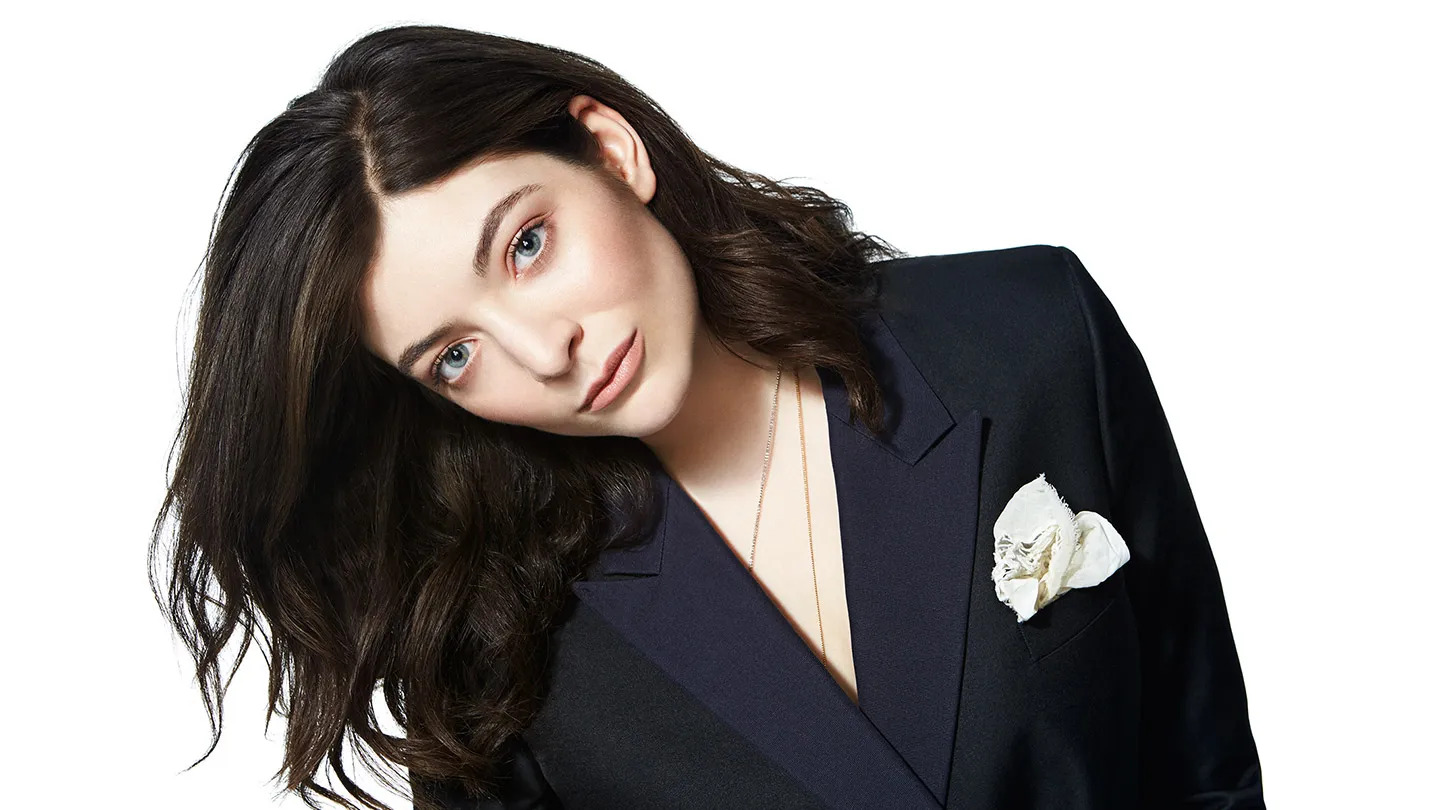
\includegraphics[height=0.5\paperheight]{te_ao_maarama/lorde.jpg} \hspace{1em}
    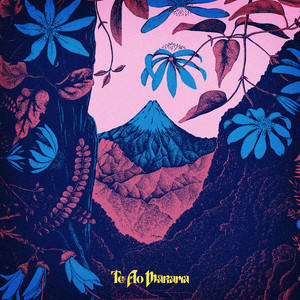
\includegraphics[height=0.5\paperheight]{te_ao_maarama/te_ao_maarama.jpg}

    \vspace{6pt}

    ``The future of music'' -- David Bowie

    \vspace{6pt}

    \tiny \href{https://www.youtube.com/watch?v=H1u0ukFst60&ab_channel=LordeVEVO}{click here for video}
\end{frame}

\begin{frame}{Leaving the group}
    \centering
    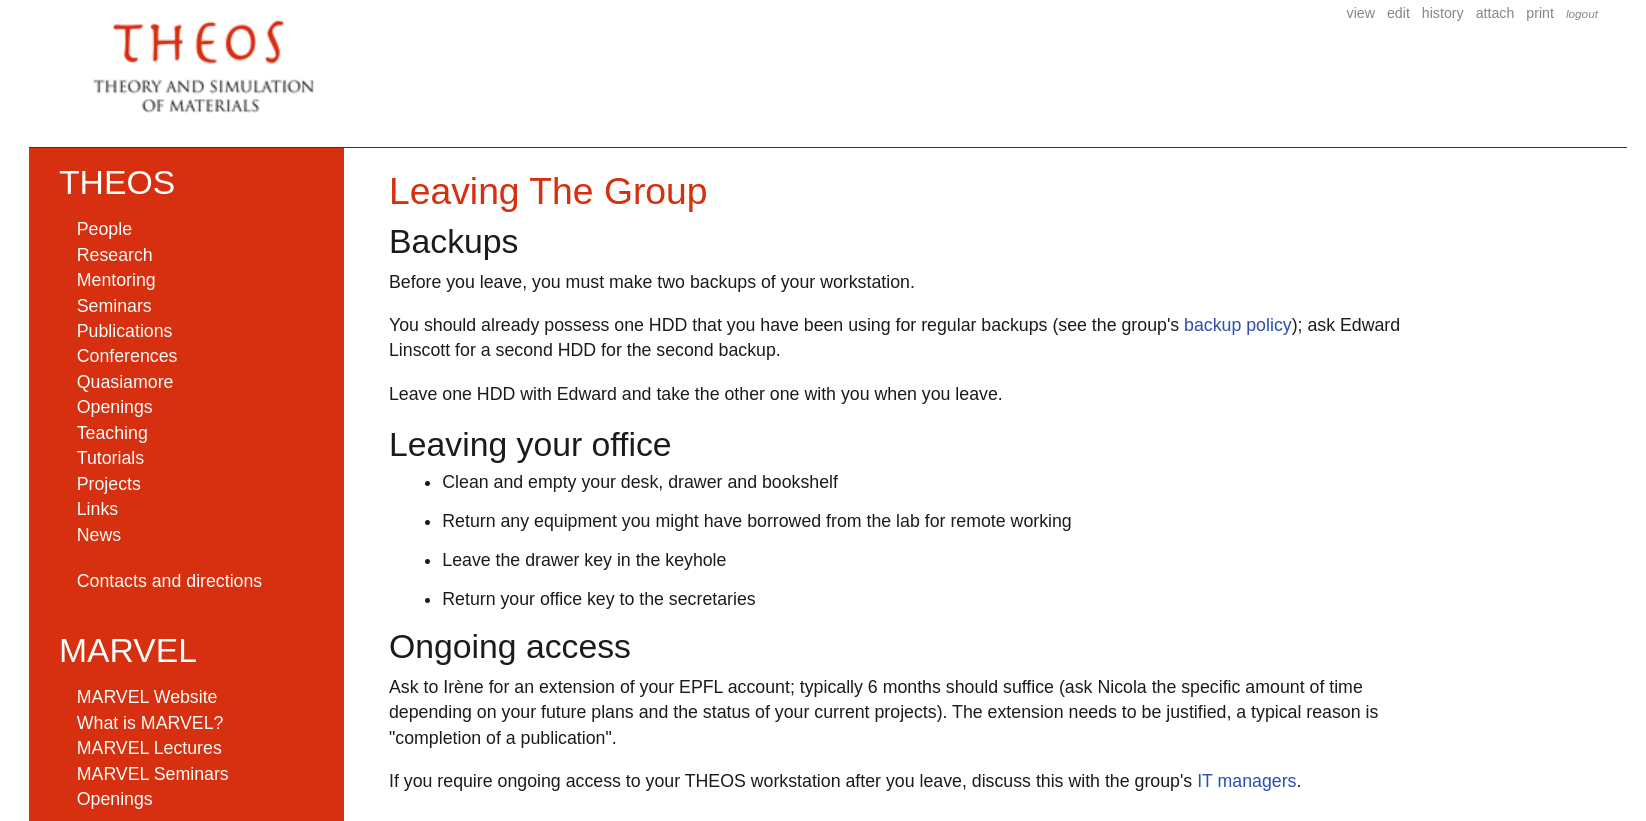
\includegraphics[width=0.9\textwidth]{figures/leaving_the_group.png}
\end{frame}

\frame{\titlepage}
% \frame{\titlepage}

\begin{frame}{DFT+\emph{U}}
    \begin{align*}
        E_\mathsf{U} = \sum_{I\sigma} \frac{U^I}{2}\Trace[\hat n^{I\sigma}(1-\hat n^{I\sigma})]
    \end{align*}
    %
    \begin{align*}
        \hat n^{I\sigma} = \hat P^I \hat \rho^\sigma \hat P^I = \sum_{i,j} \ket{\varphi^I_i}\bra{\varphi^I_i} \hat \rho^\sigma \ket{\varphi^I_j}\bra{\varphi^I_j}
    \end{align*}
    \begin{minipage}[t][0.5\paperheight][t]{\textwidth}
        \only<2>{
            \begin{center}
                \begin{tabular}{ccccc}
                    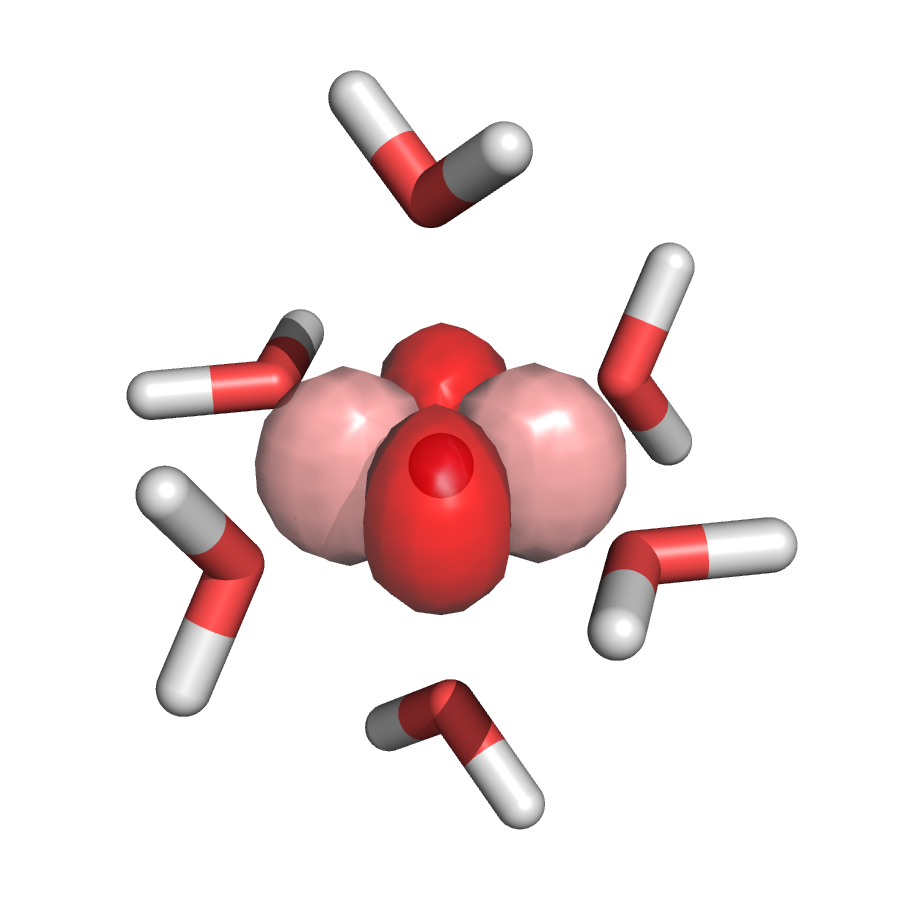
\includegraphics[trim=4cm 2cm 3cm 2cm, clip, width=0.16\textwidth]{figures/Mn3+_dxy.png} &
                    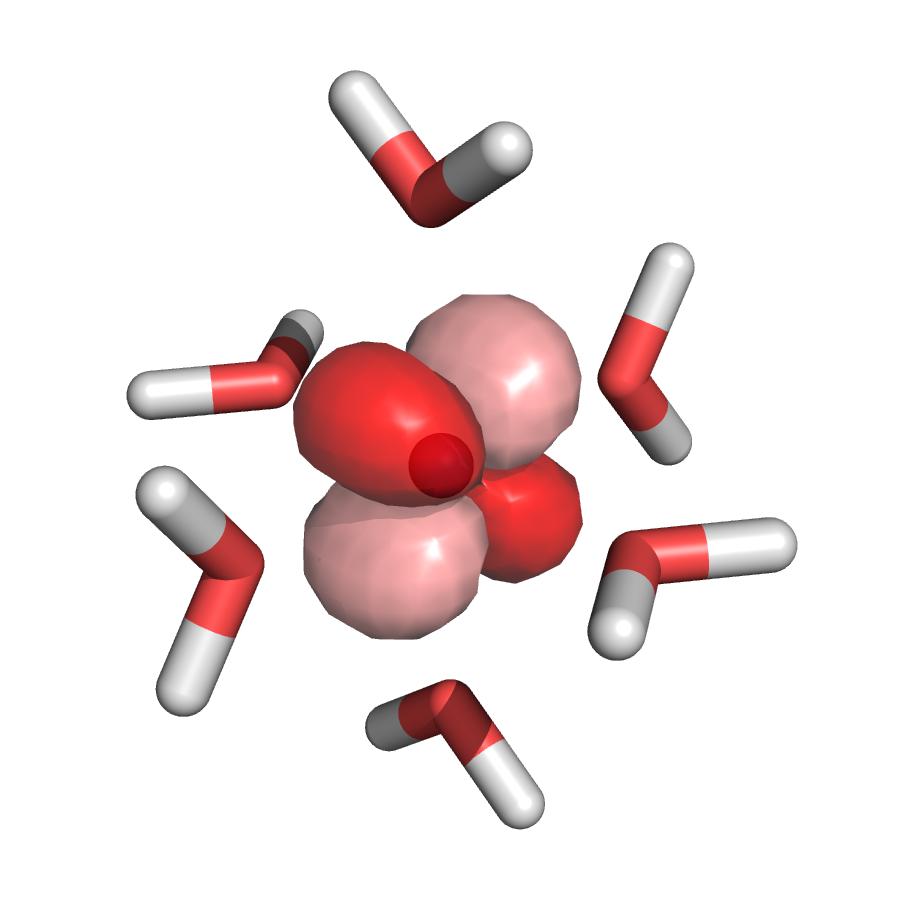
\includegraphics[trim=4cm 2cm 3cm 2cm, clip, width=0.16\textwidth]{figures/Mn3+_dxz.png} &
                    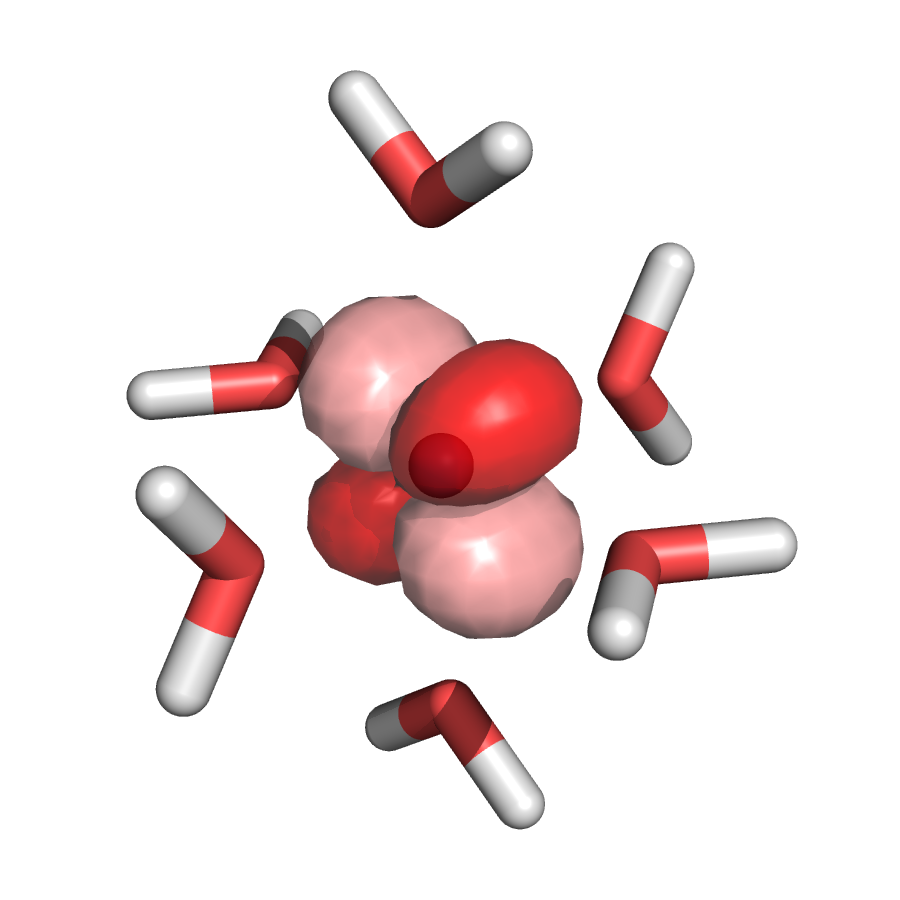
\includegraphics[trim=4cm 2cm 3cm 2cm, clip, width=0.16\textwidth]{figures/Mn3+_dyz.png} &
                    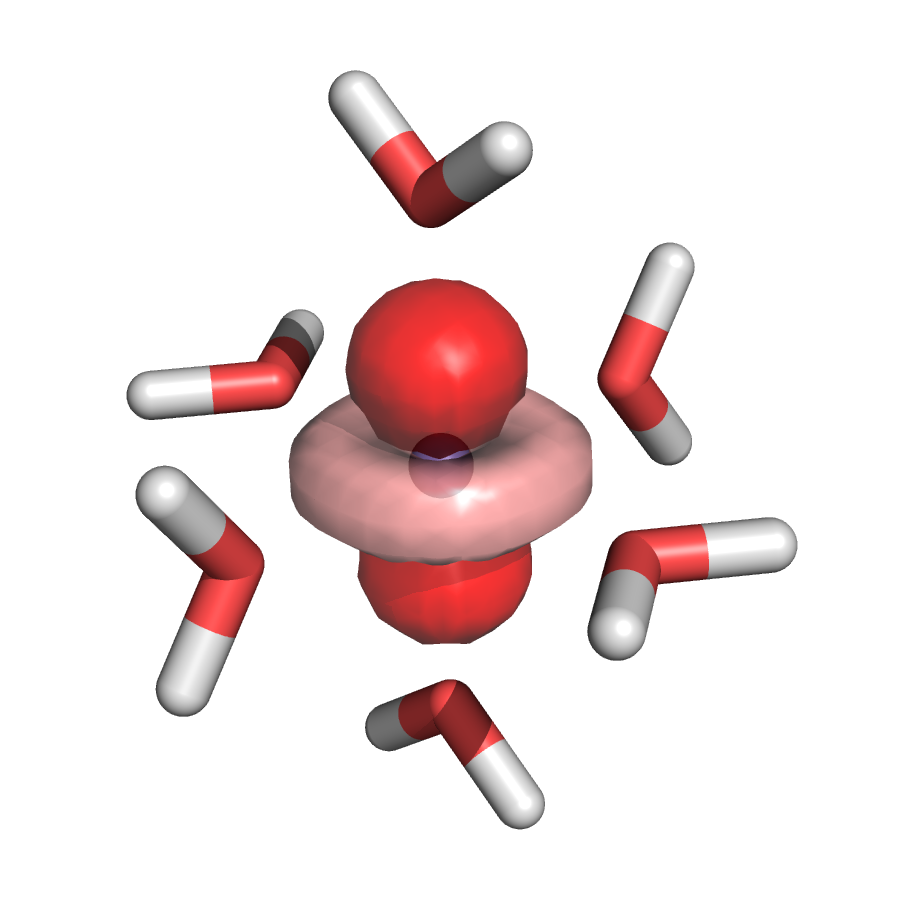
\includegraphics[trim=4cm 2cm 3cm 2cm, clip, width=0.16\textwidth]{figures/Mn3+_dz2.png} &
                    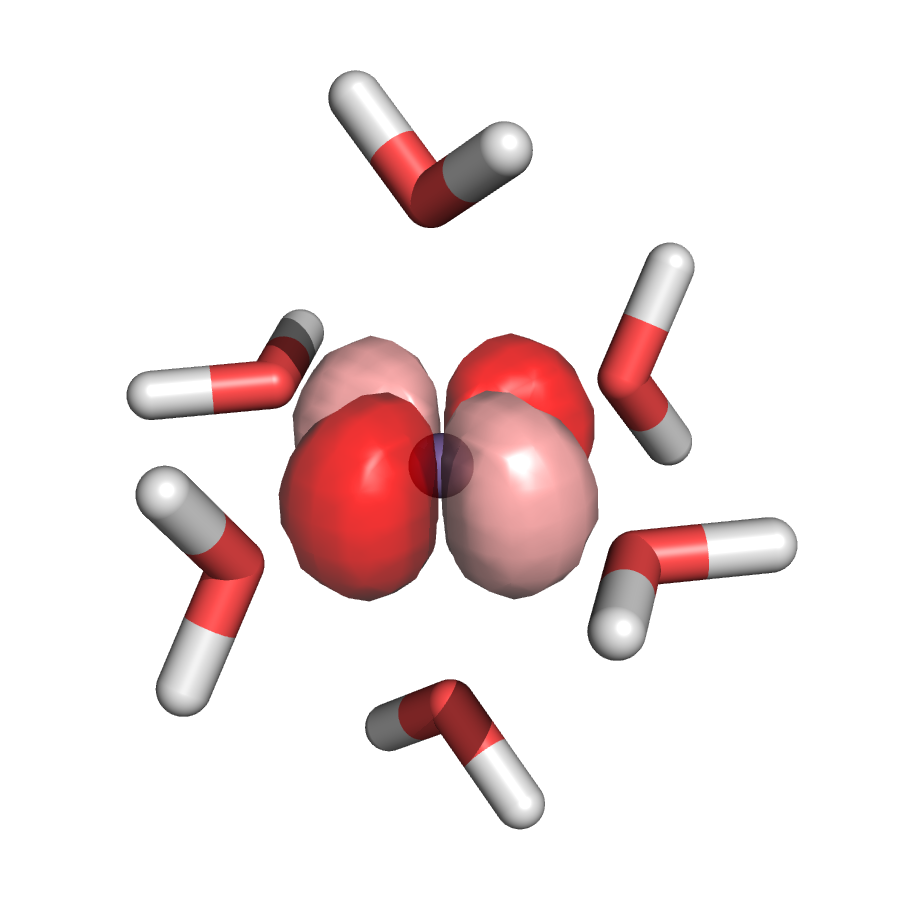
\includegraphics[trim=4cm 2cm 3cm 2cm, clip, width=0.16\textwidth]{figures/Mn3+_dx2-y2.png} \\
                    $ \braket{\mathbf{r}}{\varphi^I_1} $                                                     &
                    $ \braket{\mathbf{r}}{\varphi^I_2} $                                                     &
                    $ \braket{\mathbf{r}}{\varphi^I_3} $                                                     &
                    $ \braket{\mathbf{r}}{\varphi^I_4} $                                                     &
                    $ \braket{\mathbf{r}}{\varphi^I_5} $
                \end{tabular}
            \end{center}
        }
        %
        \only<3->{
            \begin{align*}
                \hat V_\mathsf{U} = \sum_{I\sigma ij}U^{I} \ket{\varphi^I_i}\left(\frac{1}{2}-n_{ij}^{I\sigma} \right) \bra{\varphi^I_j}
            \end{align*}
        }

        \onslide<4->{\raggedleft ... but where does this come from?}
    \end{minipage}
\end{frame}


\begin{frame}{Time for a history lesson...}
    Let's integrate the Hubbard model into the DFT framework!
    \vspace{6pt}

    \onslide<2->{
        Start with an electron-electron interaction term...
        %
        \begin{equation*}
            \hat U = \sum_{mnm'n'}\sum_{\sigma\sigma'}U_{mnm'n'}c^\dag_{m\sigma} c^\dag_{n\sigma'} c_{m'\sigma'} c_{n'\sigma},
        \end{equation*}
    }
    \onslide<3->{We make various assumptions:
        \begin{itemize}
            \item ignore all but two-site interaction terms (\`a la Hubbard model)
            \item neglect terms between opposite spin (likewise)
            \item adopt a double-counting term % (fully localised limit, all subspaces with integer occupancy)
            \item assume single-Slater-determinant wavefunction
        \end{itemize}}

    \onslide<4->{
        ... and finish with a corrective term to DFT
        %
        \begin{align*}
            E_{DFT+U}[\rho] = E_\mathsf{DFT}[\rho] + E_\mathsf{U}[\rho] = E_\mathsf{DFT}[\rho] + \sum_{I\sigma} \frac{U^I}{2}\Trace[\hat n^{I\sigma}(1-\hat n^{I\sigma})]
            \label{eqn:EU3}
        \end{align*}
    }
\end{frame}

\begin{frame}{Time for a history lesson...}

    \vspace{-3ex}
    \begin{center}
        \only<1>{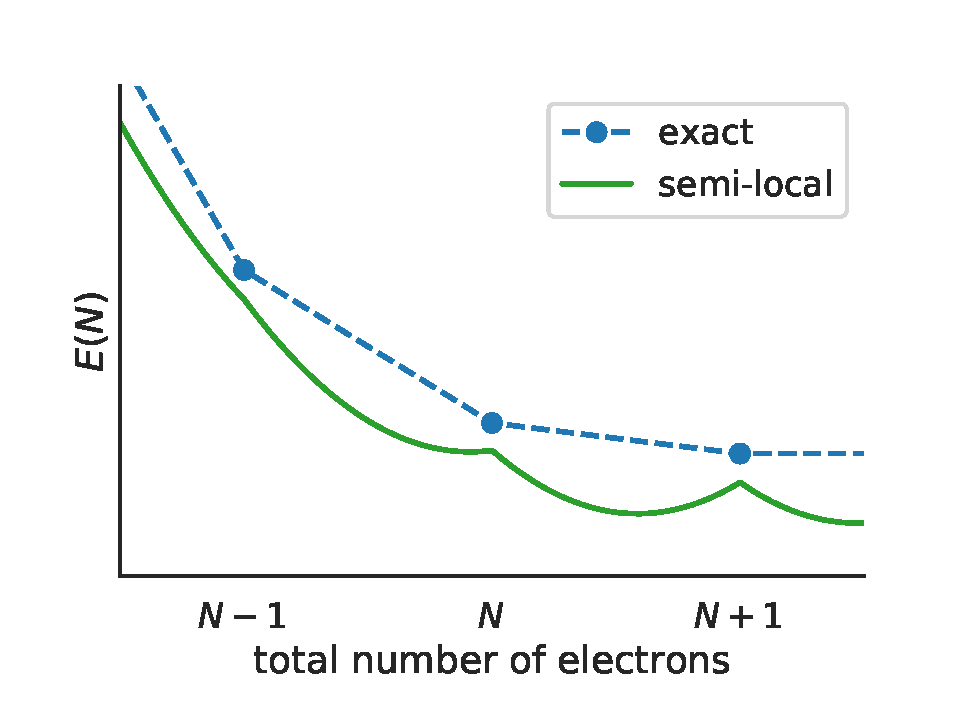
\includegraphics[height=0.5\textheight]{figures/fig_en_curve_dftu_without_correction.pdf}}
        \only<2->{
            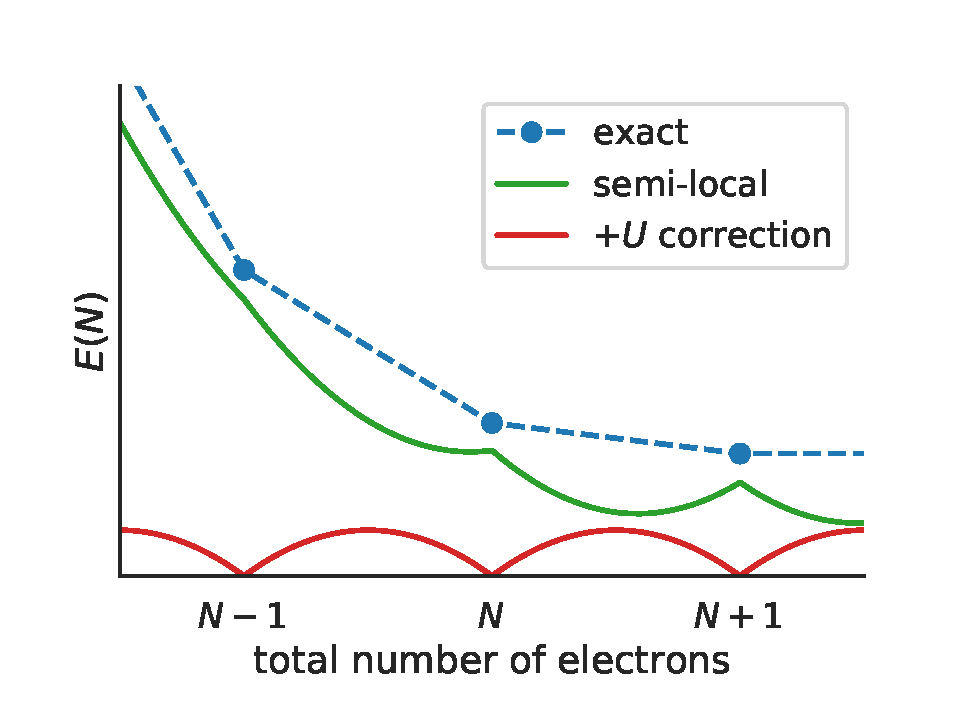
\includegraphics[height=0.5\textheight]{figures/fig_en_curve_dftu_correction.pdf}}
    \end{center}

    \small
    A modern (post hoc) interpretation:
    in a basis such that $\hat n^{I\sigma} =diag(\lambda^{I\sigma}_1, ... ,\lambda^{I\sigma}_n)$
    \begin{align*}
        E_\mathsf{U} = \sum_{I\sigma} \frac{U^I}{2}\Trace[\hat n^{I\sigma}(1-\hat n^{I\sigma})]
        = \sum_{I\sigma} \frac{U^I}{2}\sum_i \lambda^{I\sigma}_i (1-\lambda^{I\sigma}_i)
    \end{align*}
    % \begin{center}
    %    \onslide<3->{\includegraphics[height=0.4\paperheight]{../figures/fig_En_theory.pdf}} 
    % \end{center}
    \onslide<3->{We can calculate $U$ via linear response $\rightarrow$ ``self-correcting'' DFT}
    \blfootcite{Cococcioni2005a}
\end{frame}

\begin{frame}{Time for a history lesson...}
    What about DFT$+U+J$?

    \onslide<2->{

        \vspace{6pt}

        Start with an electron-electron interaction term...
        %
        \begin{equation*}
            \hat U = \sum_{mnm'n'}\sum_{\sigma\sigma'}U_{mnm'n'}c^\dag_{m\sigma} c^\dag_{n\sigma'} c_{m'\sigma'} c_{n'\sigma},
        \end{equation*}

        We make various assumptions:
        \begin{itemize}
            \item ignore all but two-site interaction terms (\`a la Hubbard model)
            \item \only<3->{\sout}{neglect terms between opposite spin (likewise)}
            \item adopt a double-counting term % (fully localised limit, all subspaces with integer occupancy)
            \item assume single-Slater-determinant wavefunction
        \end{itemize}

        ... and finish with a corrective term to DFT
        %
        \onslide<4->{
        \begin{align*}
            E_{DFT+U+J}[\rho] = E_\mathsf{DFT}[\rho] + \sum_{I\sigma} \frac{U^I-J^I}{2}\Trace[\hat n^{I\sigma}(1-\hat n^{I\sigma})]
            + \sum_{I\sigma} \frac{J^I}{2} \Trace[\hat n^{I\sigma} \hat n^{I-\sigma} - 2\delta_{\sigma \sigma_\mathsf{min}} n^{I\sigma}]
            \label{eqn:EU3}
        \end{align*}
        }
    }

\end{frame}

\begin{frame}{Time for a history lesson...}

    A modern interpretation of $+J$ was never concretely attempted. From Himmetoglu (2011):

    \vspace{6pt}

    \begin{center}
        \begin{tikzpicture}
            \path [fill overzoom image=figures/himmetoglu2011_quote.png, path fading=fade bottom] (0,0) rectangle (0.5\textwidth, 0.213\textwidth);
        \end{tikzpicture}
    \end{center}

    \onslide<2->{
    What is the analogue of piecewise linearity?
    }
    
    \onslide<3->{
    \begin{center}
        \textbf{Static correlation error (SCE)}
        \\
        energy should be piecewise linear with respect to magnetisation
    \end{center}
    }

    \blfootcite{Himmetoglu2011a}

\end{frame}

\begin{frame}{SIE and SCE in He\textsuperscript{x+}}
    \renewcommand{\figurename}{}
    \begin{columns}

        \column{0.45\linewidth}
        \begin{figure}[h!]
            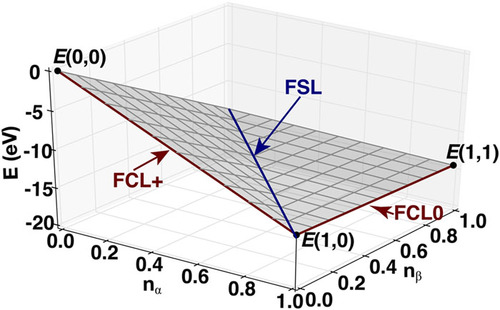
\includegraphics[width=\columnwidth]{figures/fig_bajaj_abstracted_2d_pwl.jpg}
            \caption{the flat plane}
        \end{figure}

        \column{0.4\linewidth}
        \begin{figure}
            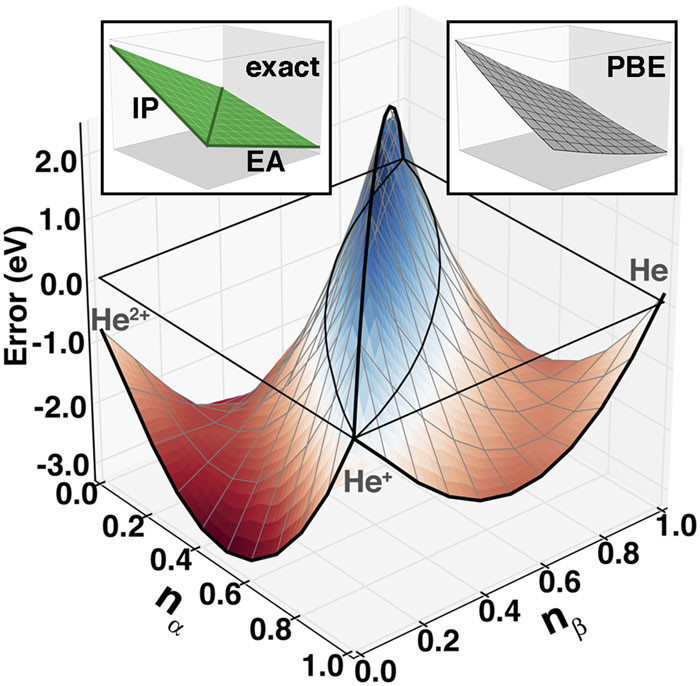
\includegraphics[width=\columnwidth]{figures/fig_bajaj_2d_pwl.jpeg}
            \caption{PBE error}
        \end{figure}

    \end{columns}
    \blfootcite{Bajaj2017}

\end{frame}

\begin{frame}{SIE and SCE in He\textsuperscript{x+}}

    ... Does DFT + \emph{U} + \emph{J} correct SIE and SCE?

    \begin{overlayarea}{\textwidth}{0.8\textheight}
    \begin{center}
        \only<2>{
        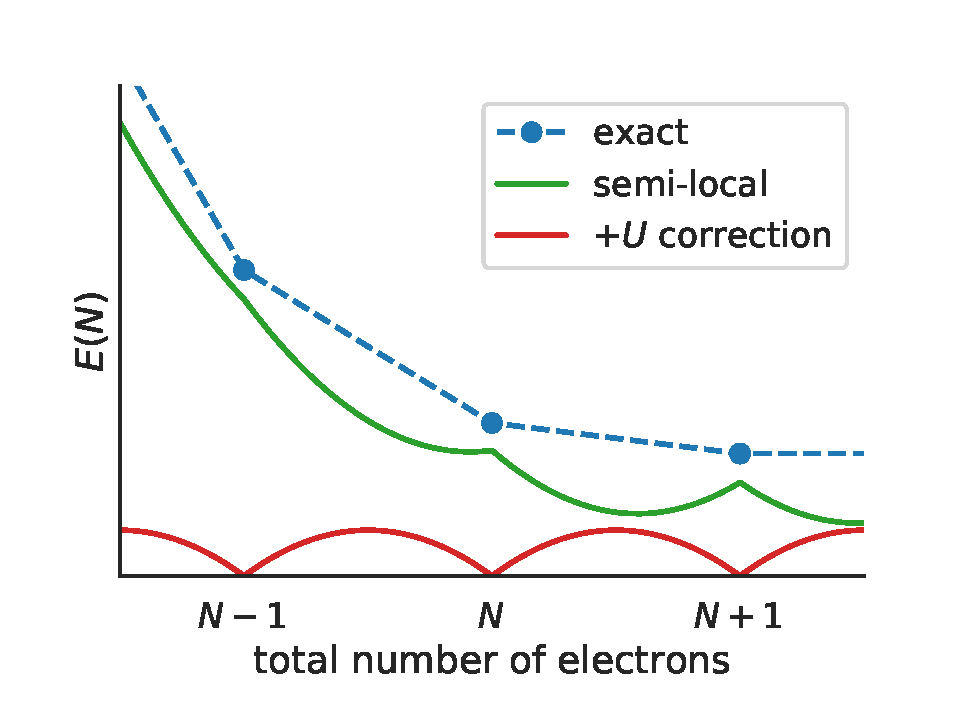
\includegraphics[width=0.5\textwidth]{figures/fig_en_curve_dftu_correction.pdf}

        \textbf{\textcolor{seaborn_green}{semi-local DFT} + \textcolor{seaborn_red}{U correction} = \textcolor{seaborn_blue}{piecewise linear}}
        }

        \only<3->{
       
        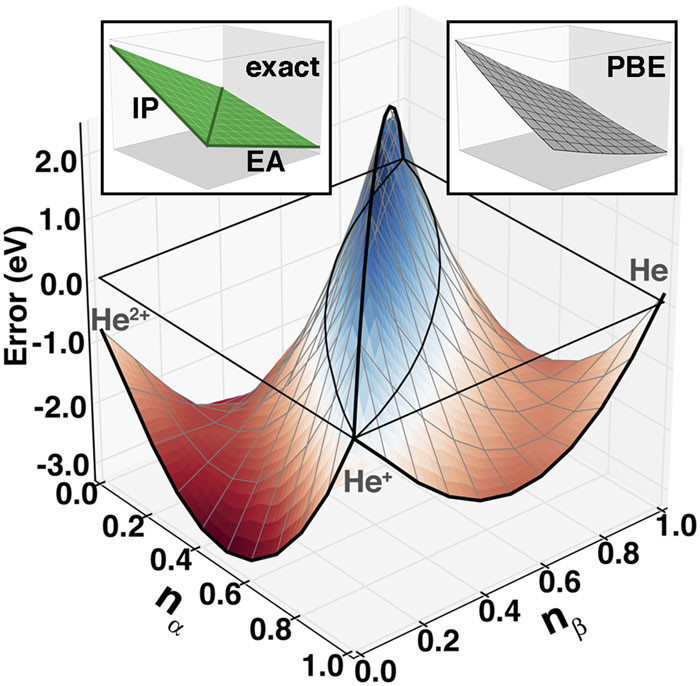
\includegraphics[width=0.4\textwidth]{figures/fig_bajaj_2d_pwl.jpeg}

            \textbf{U + J correction $\mathbf{\stackrel{?}{=}}$ flat plane $\mathbf{-}$ semi-local}
        }
        
    \end{center}
    \end{overlayarea}
    
\end{frame}
% \begin{frame}{The state of play}
%     \begin{align*}
%         E_{U} = & \sum_{I\sigma m m'} \frac{U^I}{2} \left(n^{I\sigma}_{mm'} (\delta_{m'm} - n^{I\sigma}_{m'm})\right) \label{eqn:u_correction}                              \\
%         E_{J} = & \sum_{I\sigma m m'} \frac{J^I}{2} \left( n^{I\sigma}_{mm'} n^{I-\sigma}_{m'm} - 2\delta_{\sigma \sigma_\mathrm{min}}\delta_{mm'} n^{I\sigma}_{m'm}\right)
%     \end{align*}
% \end{frame}

\begin{frame}{The +\,\emph{U} correction}
    \begin{columns}
        \column{0.5\linewidth}
        \begin{figure}[h!]
            \only<1>{
                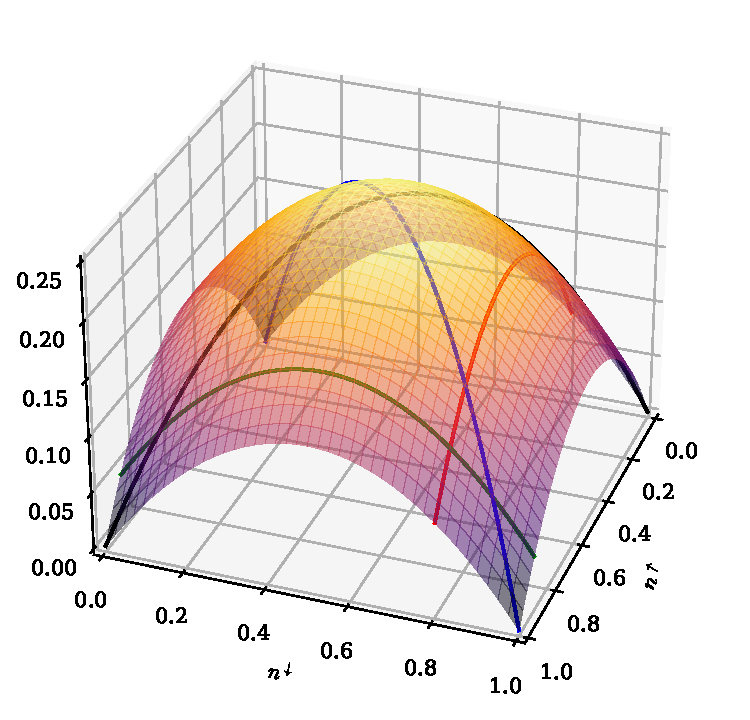
\includegraphics[width=0.8\columnwidth]{figures/u_correction_with_paths.pdf}
                \caption{$E_{U}(n^\uparrow,n^\downarrow)$}
            }
            \only<2>{
                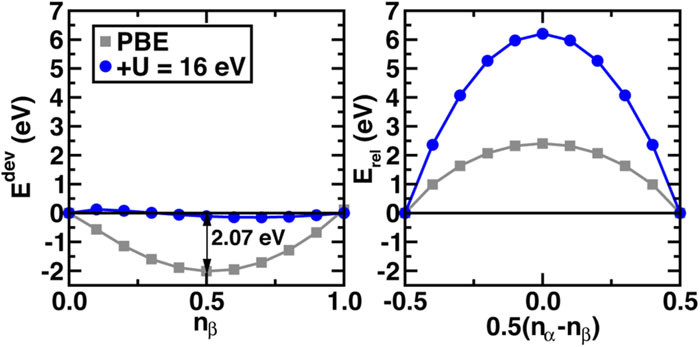
\includegraphics[width=\columnwidth]{figures/fig_bajaj_u_worsens_sce.jpeg}
                \caption{He\textsuperscript{x+} (He\textsuperscript{+} to He on left; He\textsuperscript{+} on right)}
            }
        \end{figure}
        \column{0.4\linewidth}
        \small
        \begin{subequations}
            \begin{align*}
                \left.\frac{\partial^2E_{U}}{\partial n^{\uparrow 2}}\right|_{n^\downarrow} & = -U \qquad \text{(red)}             \\
                \left.\frac{\partial^2E_{U}}{\partial n^{\downarrow 2}}\right|_{n^\uparrow} & = -U \qquad \text{(green)}           \\
                \left.\frac{\partial^2E_{U}}{\partial n^2}\right|_{\mu}                     & = -\frac{U}{2} \qquad \text{(blue)}  \\
                \left.\frac{\partial^2E_{U}}{\partial \mu^2 }\right|_{n}                    & = -\frac{U}{2} \qquad \text{(black)}
            \end{align*}
        \end{subequations}
    \end{columns}
    %
    \blfootcite{Bajaj2017}
\end{frame}
% % 
% % The $+U$ correction introduces a spin-symmetric curvature with respect to $n^\sigma$, but also adds curvature with respect to $\mu$. For semi-local functionals $\frac{d^2E}{d\mu^2}$ is already erroneously \emph{concave}, and thus $+U$ corrections worsen static correlation error \cite{Bajaj2017}.
% % 
\begin{frame}{The +\,\emph{J} correction}
    \begin{columns}
        \column{0.6\linewidth}
        \begin{figure}[h!]
            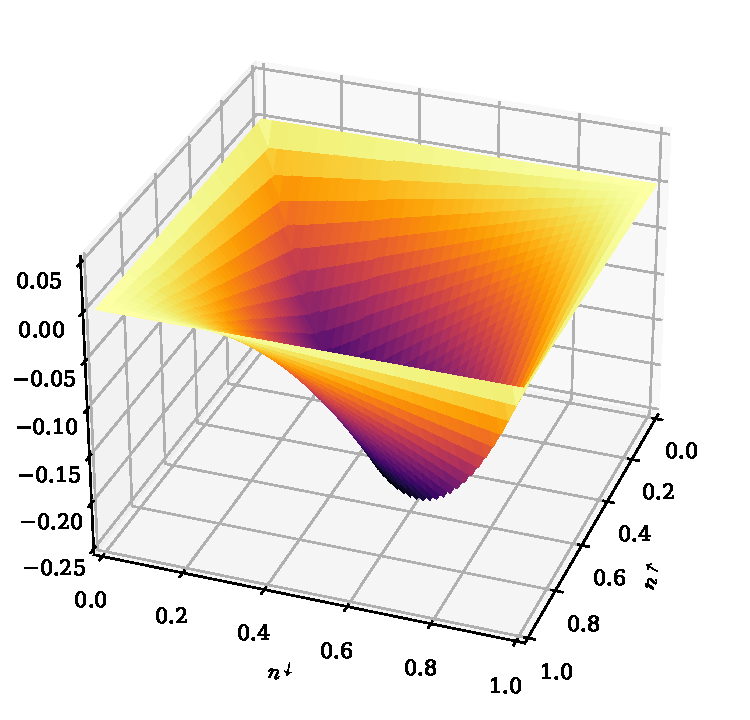
\includegraphics[width=0.7\columnwidth]{figures/j_correction.pdf}
            \caption{$E_{J}(n^\uparrow,n^\downarrow)$}
            \label{fig:j_correction}
        \end{figure}
        \column{0.35\linewidth}
        %
        \footnotesize
        \begin{subequations}
            \begin{align*}
                \left.\frac{\partial^2E_{J}}{\partial n^2}\right|_{\mu}                     & = \frac{J}{2}                                 \\
                \left.\frac{\partial^2E_{J}}{\partial\mu^2}\right|_{n}                      & = -\frac{J}{2} \qquad \text{ for } \mu \neq 0 \\
                \left.\frac{\partial^2E_{J}}{\partial n^{\uparrow 2}}\right|_{n^\downarrow} & = 0                                           \\
                \left.\frac{\partial^2E_{J}}{\partial n^{\downarrow 2}}\right|_{n^\uparrow} & = 0
            \end{align*}
        \end{subequations}

        Not even the right shape!
    \end{columns}
\end{frame}
% % 
% % \subsection{Should we use $U$ or $U_\mathrm{eff} = U - J$?}
% % 
% % \begin{figure}[h!]
% %     \begin{subfigure}[b]{0.4\columnwidth}
% %         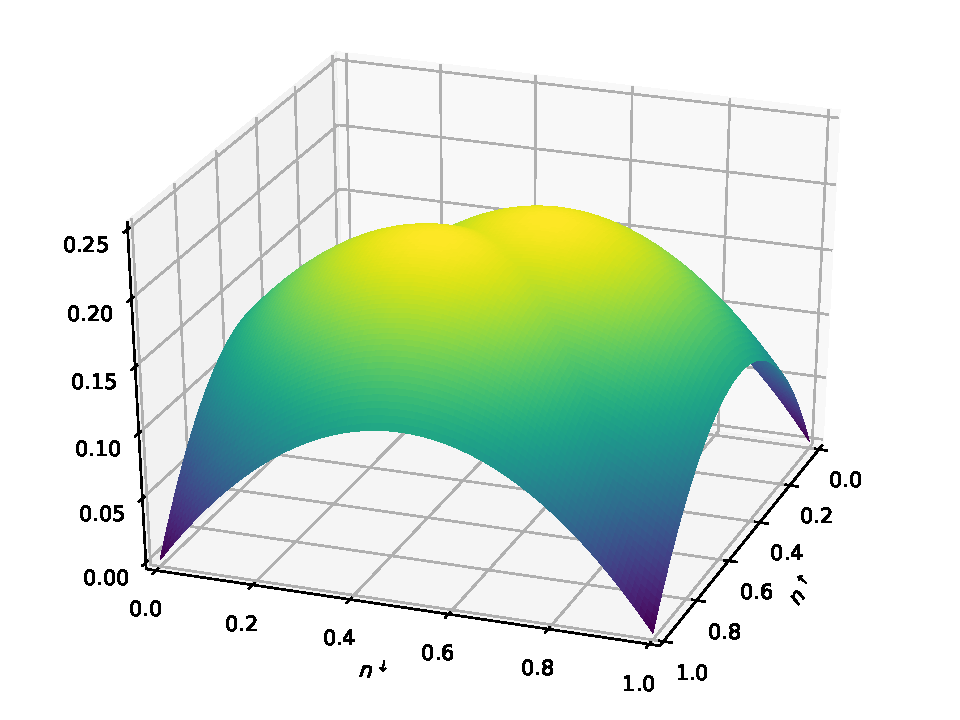
\includegraphics[width=\columnwidth]{figures/u_j_correction.pdf}
% %         \caption{with a $E_U$ prefactor of $U - J$}
% %         \label{fig:u_j_correction}
% %     \end{subfigure}
% %     \begin{subfigure}[b]{0.4\columnwidth}
% %         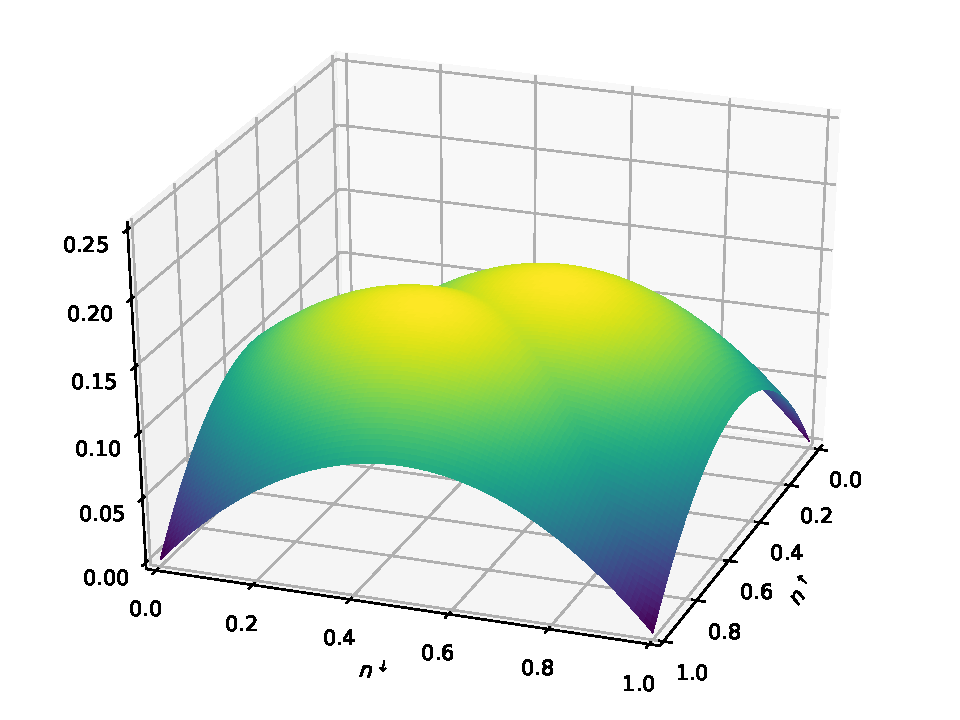
\includegraphics[width=\columnwidth]{figures/ueff_j_correction.pdf}
% %         \caption{with a $E_U$ prefactor of $U$}
% %         \label{fig:ueff_j_correction}
% %     \end{subfigure}
% %     % \begin{subfigure}[b]{0.4\columnwidth}
% %     %     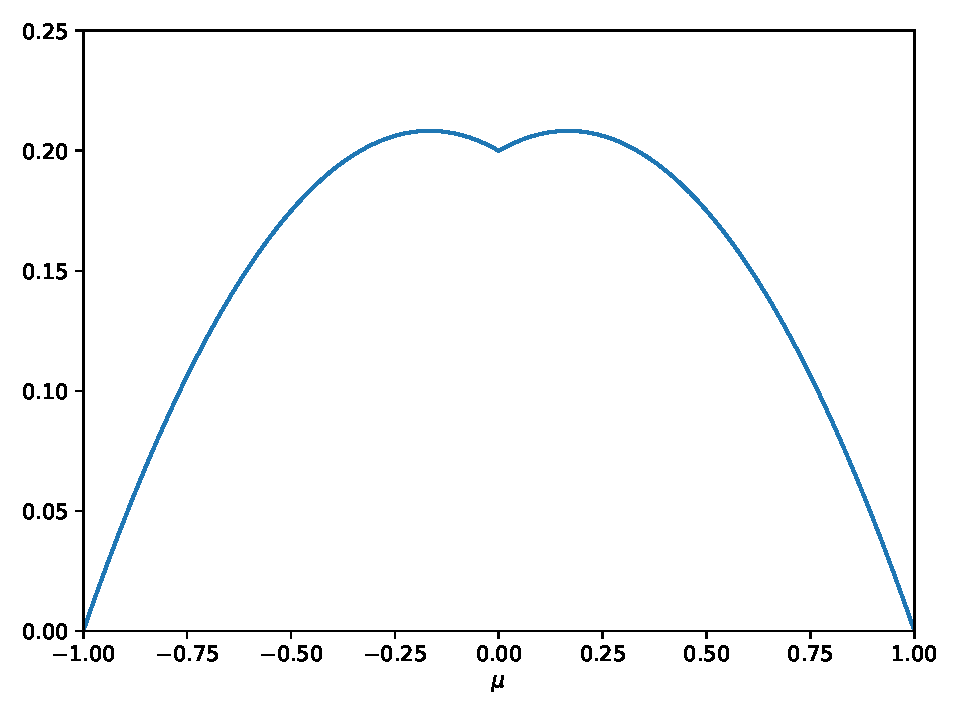
\includegraphics[width=\columnwidth]{figures/u_j_correction_2d.pdf}
% %     %     \caption{cross-section of \cref{fig:u_j_correction} along $n=1$}
% %     %     \label{fig:u_j_correction_2d}
% %     % \end{subfigure}
% %     % \begin{subfigure}[b]{0.4\columnwidth}
% %     %     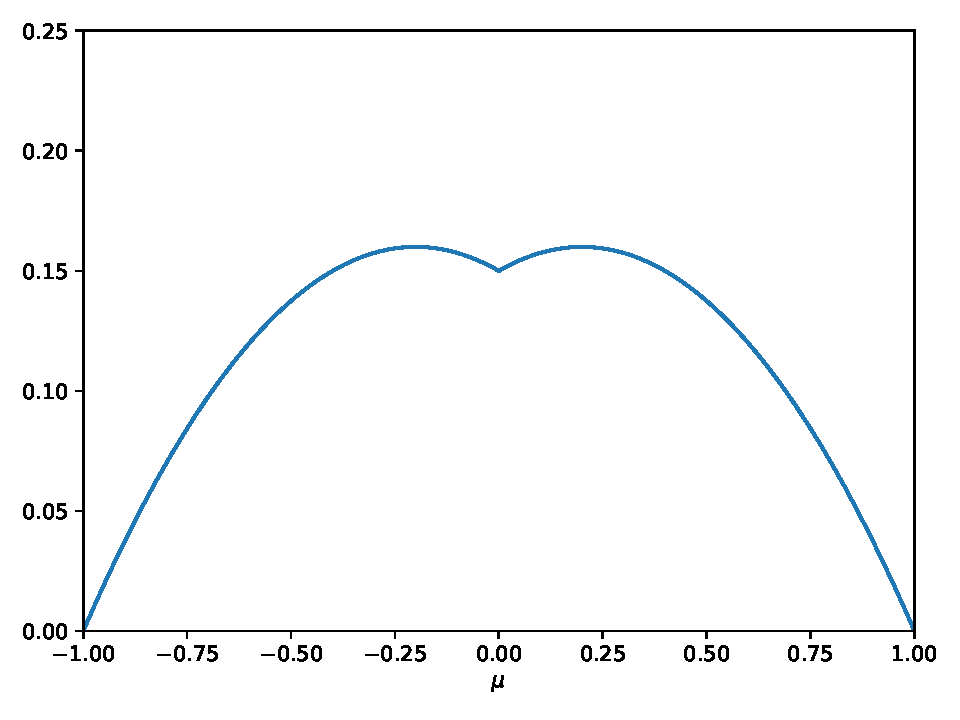
\includegraphics[width=\columnwidth]{figures/ueff_j_correction_2d.pdf}
% %     %     \caption{cross-section of \cref{fig:ueff_j_correction} along $n=1$}
% %     %     \label{fig:ueff_j_correction_2d}
% %     % \end{subfigure}
% %     \caption{The corrective surface $E_U(n^\uparrow, n^\downarrow) + E_J(n^\uparrow, n^\downarrow)$, for $J = 0.2U$}
% %     \label{fig:u_vs_ueff}
% % \end{figure}
% % %
% % \noindent Often the prefactor to the +\,\emph{U} correction is rendered as $U_\mathrm{eff} = U - J$. In this framework, if we want to apply some value for $J$ to our system we should simultaneously reduce the prefactor of the +\,\emph{U} correction by the same amount.
% % 
\begin{frame}{The combined correction}
    \footnotesize
    \begin{columns}
        \column{0.45\linewidth}
        $U_\mathsf{eff} = U - J$:
        \begin{subequations}
            \begin{align*}
                \left.\frac{\partial^2}{\partial n^2}\right|_{\mu} (E_{U_\mathsf{eff}} + E_J)                     & = -\frac{U-2J}{2}                            \nonumber  \\
                \left.\frac{\partial^2}{\partial \mu^2}\right|_{n} (E_{U_\mathsf{eff}} + E_J)                     & = -\frac{U}{2} \qquad \text{ for } \mu \neq 0 \nonumber \\
                \left.\frac{\partial^2}{\partial n^{\uparrow 2}}\right|_{n^\downarrow} (E_{U_\mathsf{eff}} + E_J) & = -(U - J) \qquad \text{ for } \mu \neq 0     \nonumber \\
                \left.\frac{\partial^2}{\partial n^{\downarrow 2}}\right|_{n^\uparrow} (E_{U_\mathsf{eff}} + E_J) & = -(U - J) \qquad \text{ for } \mu \neq 0\nonumber
            \end{align*}
            \label{eqn:2nd_derivatives_ueff_plus_j}
        \end{subequations}
        \column{0.45\linewidth}
        $U_\mathsf{eff} = U$:
        \begin{subequations}
            \begin{align*}
                \left.\frac{\partial^2}{\partial n^2}\right|_{\mu} (E_{U} + E_J)                     & = -\frac{U-J}{2}                                \nonumber \\
                \left.\frac{\partial^2}{\partial \mu^2}\right|_{n} (E_{U} + E_J)                     & = -\frac{U+J}{2} \qquad \text{ for } \mu \neq 0 \nonumber \\
                \left.\frac{\partial^2}{\partial n^{\uparrow 2}}\right|_{n^\downarrow} (E_{U} + E_J) & = -U \qquad \text{ for } \mu \neq 0             \nonumber \\
                \left.\frac{\partial^2}{\partial n^{\downarrow 2}}\right|_{n^\uparrow} (E_{U} + E_J) & = -U \qquad \text{ for } \mu \neq 0\nonumber
            \end{align*}%
            \label{eqn:2nd_derivatives_u_plus_j}%
        \end{subequations}%
    \end{columns}
    %
\end{frame}
% % %
% % These two approaches are also plotted in \cref{fig:u_vs_ueff}. We can see immediately there are a number of issues with using $U_\mathrm{eff}$. All bar one of these curvature corrections is parametrised by a mix of $U$ and $J$ -- and bizarrely the one that is parametrised solely by $U$ is the curvature with respect to $\mu$!
% % 
% % Using $U$ rather than $U_\mathrm{eff}$ (\cref{eqn:2nd_derivatives_u_plus_j}) is not much better, with the curvature with respect to $n$ and $\mu$ being a function of both $U$ and $J$. At least in this scheme, the derivatives with respect to $n^\sigma$ are parametrised by $U$ alone. Thus \textbf{using $U$ rather than $U_\mathrm{eff}$ is a better (if imperfect) choice} when performing DFT\,+\,$U$\,+\,$J$.
% % 
% % \subsection{What to do with the minority spin term?}
% \begin{frame}{Excluding the minority spin}
%     \footnotesize
%     \vspace{-1em}
%     \begin{align}
%         E_{J} = & \sum_{I\sigma m m'} \frac{J^I}{2} \left( n^{I\sigma}_{mm'} n^{I-\sigma}_{m'm} - 2\delta_{\sigma \sigma_\mathrm{min}}\delta_{mm'} n^{I\sigma}_{m'm}\right)
%         \label{eqn:j_correction}
%     \end{align}
%     \begin{figure}
%         \begin{subfigure}[b]{0.4\columnwidth}
%             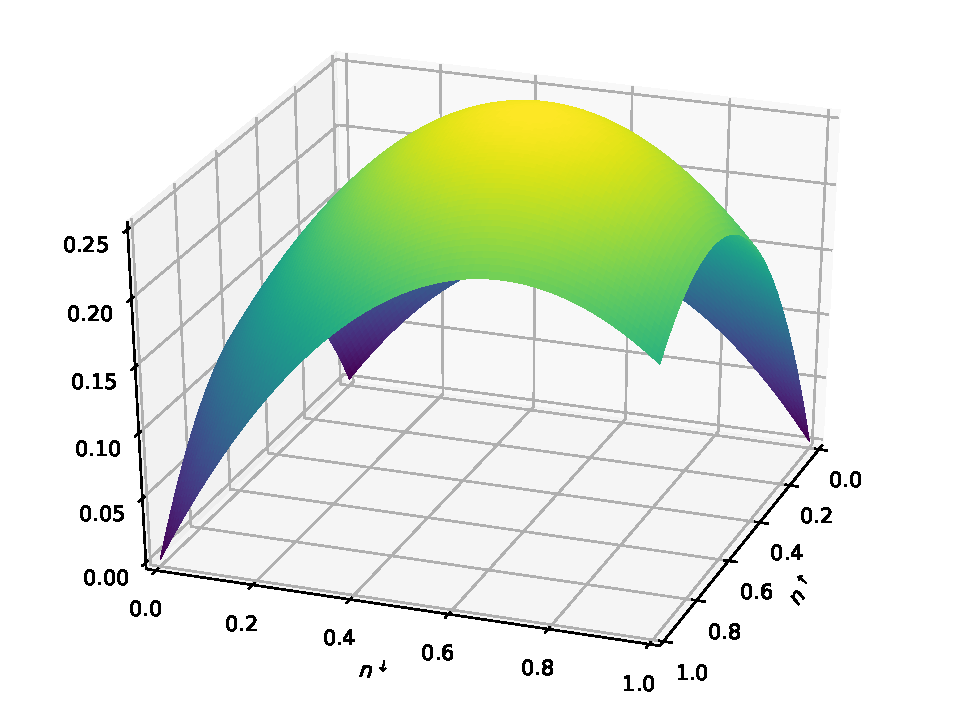
\includegraphics[width=\columnwidth]{figures/u_jnomin_correction.pdf}
%             \caption{with a $E_U$ prefactor of $U - J$}
%             \label{fig:u_jnomin_correction}
%         \end{subfigure}
%         \begin{subfigure}[b]{0.4\columnwidth}
%             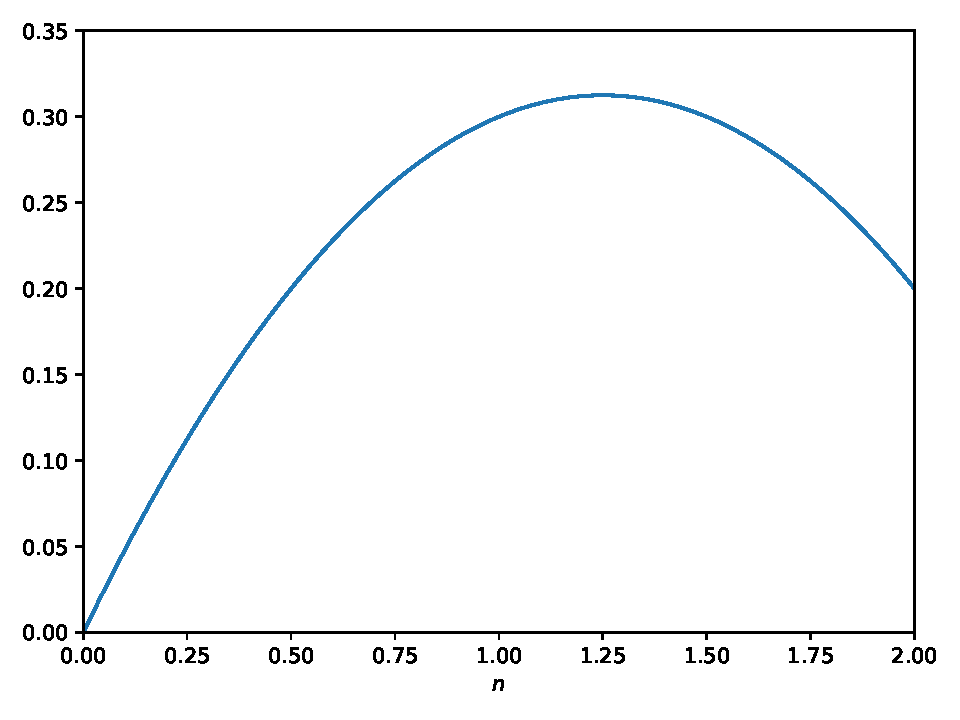
\includegraphics[width=\columnwidth]{figures/u_jnomin_correction_2d.pdf}
%             \caption{Cross-section along $\mu=0$}
%             \label{fig:u_jnomin_correction_2d}
%         \end{subfigure}
%         \caption{The corrective surface $E_U(n^\uparrow, n^\downarrow) + E_J(n^\uparrow, n^\downarrow)$, for $J = 0.2U$, where $E_J$ does not include the minority spin term.}
%         \label{fig:j_vs_jnomin}
%     \end{figure}
% \end{frame}
% 
% Sometimes the ``minority spin term" in the $+J$ correction\footnote{that is, the second term in \cref{eqn:j_correction}} is dropped because it can lead to numerical difficulties. However, this leads to a much more grevious error: the $+J$ correction without this term is non-vanishing when both spin channels are filled (see \cref{fig:j_vs_jnomin}). This is the case regardless of whether the Hubbard correction prefactor is $U$ or $U_\mathrm{eff} = U - J$.
% 
% The general philosophy of Hubbard corrections is that we trust DFT to provide reliable energies at integer numbers of electrons,\footnote{For the moment I will be vague as to what occupancies I am talking about, although it's always worth keeping in mind that local occpuancies $n = \trace{n^{\sigma}_{mm'}}$ of Hubbard subspaces are very different from the total occupancy of the entire system $N$.} and any correction to the DFT energy should vanish at these points. It follows that \textbf{this minority spin term must not be dropped} and instead these numerical difficulties should be tolerated or somehow overcome.
% 
% \section{Criteria for sensible Hubbard-like corrections}
% \noindent The goal of this work is to devise a new Hubbard-like correction to address self-interaction error (SIE) and static correlation error (SCE). At this point there are several philosophical choices one can make. Based on our above study of the DFT\,+\,$U$\,+\,$J$ here are the properties I would like my functional to possess:
% 
\begin{frame}{Rethinking inter-spin corrections}
    \begin{align*}
        E_{U} = & \sum_{I\sigma m m'} \frac{U^I}{2} \left(n^{I\sigma}_{mm'} (\delta_{m'm} - n^{I\sigma}_{m'm})\right)                                                       \\
        E_{J} = & \sum_{I\sigma m m'} \frac{J^I}{2} \left( n^{I\sigma}_{mm'} n^{I-\sigma}_{m'm} - 2\delta_{\sigma \sigma_\mathsf{min}}\delta_{mm'} n^{I\sigma}_{m'm}\right)
        \label{eqn:j_correction}
    \end{align*}
    Observations on conventional DFT\,+\,$U$ and DFT\,+\,$U$\,+\,$J$
    \begin{itemize}
        \item the correction is not the right shape
        \item lots of inter-dependence
        \item (minority $J$ term is important)
    \end{itemize}

    Principles for designing a new Hubbard-like correction (i.e. quadratic in $\hat n$)
    \begin{enumerate}
        \item decouple our treatment of SIE and SCE
        \item vanishing at integer occupancies
        \item be continuous
    \end{enumerate}
\end{frame}
% %
% Finally, the correction I will construct will simply be designed to fit the shape of the errors we are trying to address, without reference to some sort of physical model. We all know that historically the Hubbard correction was (somewhat arbitrarily) derived from the Hubbard model. I do not think this is the right approach. Instead, I believe that it is much better to be pragmatic, and, in the spirit of Matteo's 2005 paper, simply choose a corrective term that best addresses the errors we are trying to correct: that is (a) quadratic corrections to the energy in terms of the occupancies of individual orbitals and (b) quadratic corrections to the energy in terms of the magnetic moment of individual orbitals.
% 
% \section{The novel functionals}
% \subsection{A novel correction for SIE}
% Here is my first proposed energy correction for our \emph{1s} system, first attempting to address self-interaction error:
% 
\begin{frame}{Correction to SIE}
    \begin{equation*}
        % E_1(\{U^\sigma\}, \{n^\sigma\}) = \sum_\sigma \frac{U^\sigma}{4} \left(|\tilde n| + \tilde n(1 - 2n^\sigma)\right)
        \sum_\sigma \frac{U^\sigma}{2} \left(n^\uparrow + n^\downarrow - 1\right) \times
        \begin{cases}
            -n^\sigma    & n < 1 \\
            1 - n^\sigma & n > 1
        \end{cases}
    \end{equation*}
    %
    \begin{figure}[t!]
        \begin{subfigure}[b]{0.4\columnwidth}
            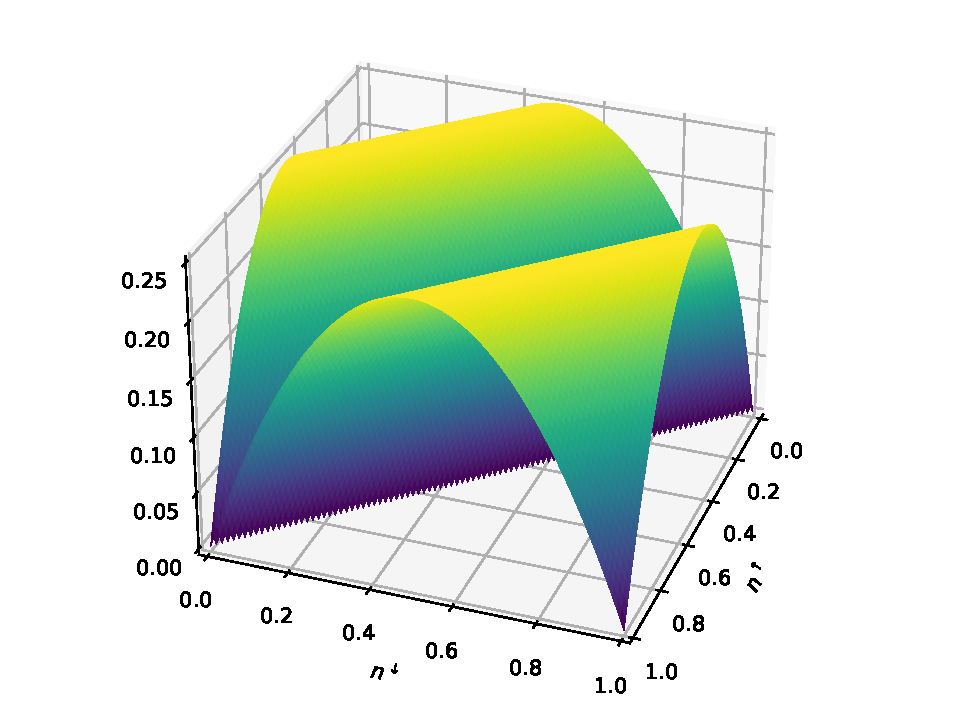
\includegraphics[width=\columnwidth]{figures/novel_u_correction_equal.pdf}
            \caption{$U^\uparrow = U^\downarrow$}
        \end{subfigure}
        \begin{subfigure}[b]{0.4\columnwidth}
            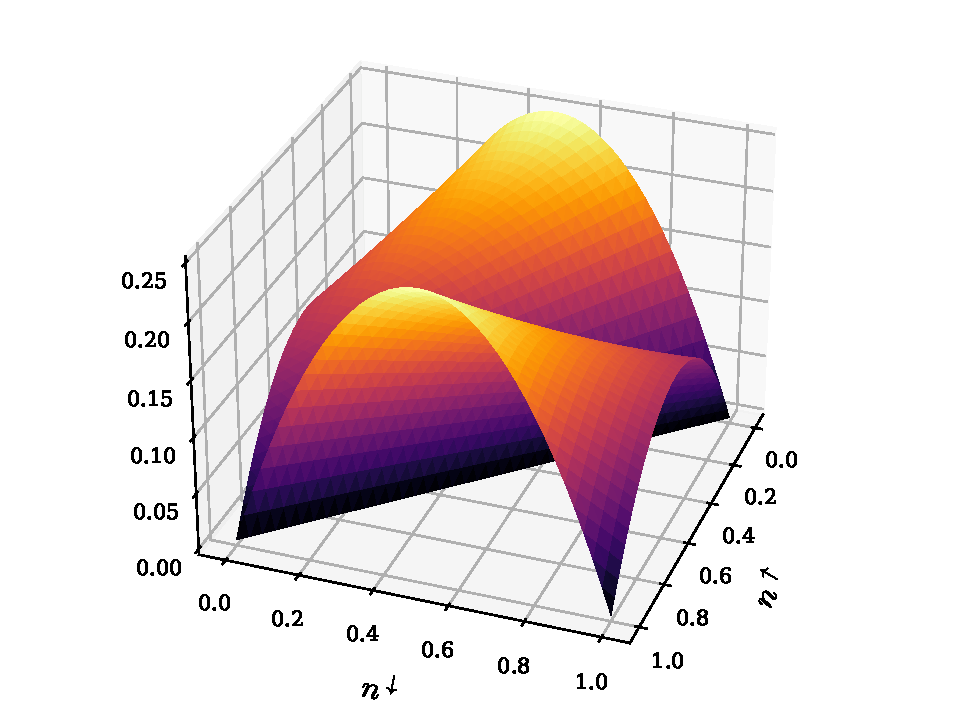
\includegraphics[width=\columnwidth]{figures/novel_u_correction.pdf}
            \caption{$U^\uparrow = U^\downarrow/2$}
        \end{subfigure}
    \end{figure}
\end{frame}
% % %
% % The notable properties of this functional are as follows
% % %
\begin{frame}{Correction to SIE}
    \begin{columns}
        \column{0.38\linewidth}
        \centering
        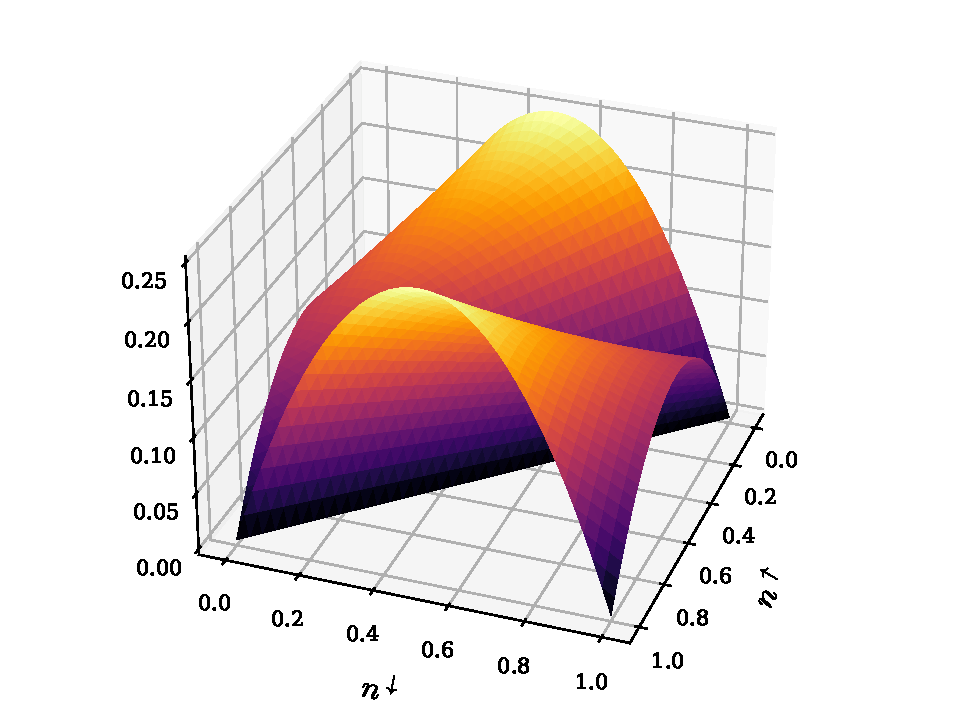
\includegraphics[width=1\columnwidth]{figures/novel_u_correction.pdf}
        \column{0.58\linewidth}
        \footnotesize
        \begin{enumerate}
            \item it is zero for integer numbers of electrons
            \item the curvature with respect to $n^\sigma$ is entirely controlled by $U^\sigma$, i.e.
                  \begin{equation*}
                      \left.\frac{\partial^2 E_1}{\partial n^{\sigma 2}}\right|_{n^{-\sigma}} = - U^\sigma
                  \end{equation*}
            \item the curvature with respect to $\mu$ is \emph{untouched} by this correction
                  \begin{equation*}
                      \left.\frac{\partial^2 E_1}{\partial \mu^{2}}\right|_{n} = 0
                  \end{equation*}
                  which would imply that this correction will selectively address SIE and not SCE
            \item the curvature with respect to the total occupancy $n = n^\uparrow + n^\downarrow$ is given by the average
                  \begin{equation*}
                      \left.\frac{\partial^2 E_1}{\partial n^{2}}\right|_{\mu} = -\frac{U^\uparrow + U^\downarrow}{2}
                  \end{equation*}
                  % I would argue that this curvature is less important (after all, derivatives with respect to $n^\sigma$ not $n$ give rise to the eigenenergies $\varepsilon^\sigma$) but nevertheless it is comforting that this second derivative is (a) constant everywhere and (b) is an intuitive value
        \end{enumerate}
    \end{columns}
\end{frame}
% % %
% % Of course, we do now have a discontinuity at $\tilde n = 0$. It remains to be seen if this will lead to numerical difficulties. It is not possible to construct this functional without this discontinuity while retaining the above properties.
% % 
% % % In order to generalise \cref{eqn:novel_u_correction} to a multi-orbital Hubbard site, I imagine the path forward is to work with the set of orbitals that diagonalise $n_{mm'}$, but I need to give this more thought as there are some subtleties.\footnote{e.g. $n_{mm'}$, $n_{mm'}^\uparrow$, and $n_{mm'}^\downarrow$ will diagonalised by different sets of orbitals}
% % %If $\{\ket{\varphi_i}\}$ is the set of orbitals that diagonalise $n_{mm'}$ then
% % 
% % %
% % This is plotted in \cref{fig:novel_u_potential,fig:novel_u_potential_2d}. The first term in this correction is very familiar -- it is simply the conventional +\emph{U} potential $\hat v = \sum_{i\sigma} U (\frac{1}{2} - n^\sigma_i)\ket{i}\bra{i}$ with a spin-dependent $U$! The second term is novel.
% % 
% % \subsection{A novel correction for SCE}
% % Here is my second proposed energy correction for our \emph{1s} system, now attempting to address static correlation error:
% % %
\begin{frame}{Correction to SCE}
    \vspace{-1em}
    \begin{equation*}
        % E_2(J, \{n^\sigma\}) % = & \frac{K}{4}\left[(n^\uparrow-n^\downarrow)^2-(|\tilde n|-1)^2\right] \nonumber \\
        % = & \frac{K}{4}\left[(n^\uparrow)^2 - 2n^\uparrow n^\downarrow + (n^\downarrow)^2-(n^\uparrow + n^\downarrow - 1)^2 + 2(|n^\uparrow + n^\downarrow - 1|) -1)\right] \nonumber \\
        % = & \frac{K}{2}\left[- 2 n^\uparrow n^\downarrow + n^\uparrow + n^\downarrow - 1 + (|n^\uparrow + n^\downarrow - 1|)\right] \nonumber \\
        \begin{cases}
            - Jn^\uparrow n^\downarrow            & n < 1 \\
            - J(1 - n^\uparrow)(1 - n^\downarrow) & n > 1
        \end{cases}
        \label{eqn:novel_k_correction}
    \end{equation*}
    % %
    % where I have chosen to parametrise this correction with the parameter $K$ rather than $J$ to try and avoid any connection with ideas associated with exchange coupling mechanisms; at the end of the day, this is an empirical correction to the energy curvature due to SCE, not a Hamiltonian embedded within DFT.
    % 
    % Much like my energy correction to SIE, this is an opaque expression with a very simple shape (as can be seen in \cref{fig:novel_k_correction}).
    % %
    \vspace{-1em}
    \begin{figure}[t!]
        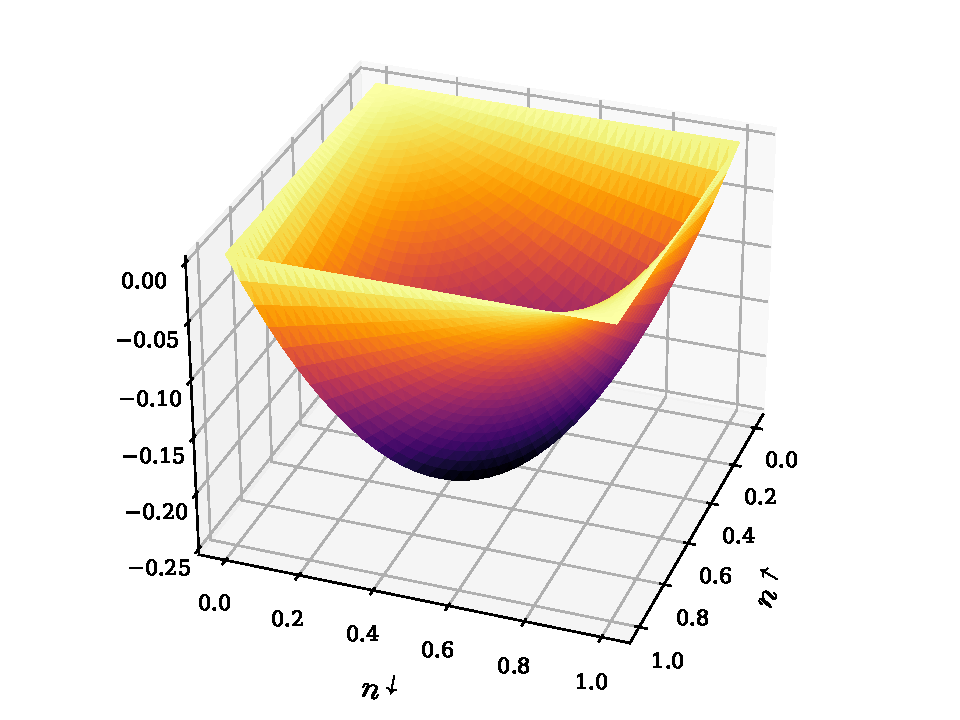
\includegraphics[width=0.5\columnwidth]{figures/novel_k_correction.pdf}
        %\caption{My proposed second correction, $E_2(K, \{n^\sigma\})$ for addressing SCE, with $K = 1$}
        \label{fig:novel_k_correction}
    \end{figure}
\end{frame}
% %
\begin{frame}{Correction to SCE}
    \begin{columns}
        \column{0.38\linewidth}
        \centering
        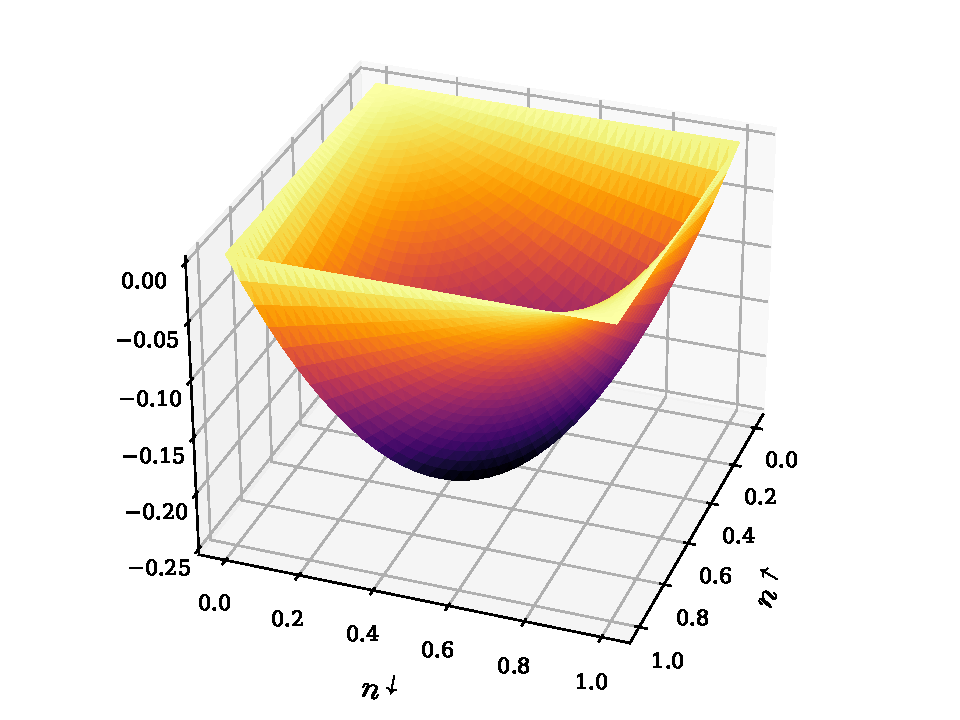
\includegraphics[width=1.2\columnwidth]{figures/novel_k_correction.pdf}
        \column{0.58\linewidth}
        \footnotesize
        This second energy correction term possesses the following important properties:
        %
        \begin{enumerate}
            \item it is zero for integer numbers of electrons
            \item the curvature with respect to $\mu$ is controlled by the parameter $J$
                  \begin{equation*}
                      \left.\frac{\partial^2 E_2}{\partial \mu^{2}}\right|_{n} = \frac{J}{2}
                  \end{equation*}
            \item the curvature with respect to $n^\sigma$ is zero
                  \begin{equation*}
                      \left.\frac{\partial^2 E_2}{\partial n^{\sigma 2}}\right|_{n^{-\sigma}} = 0
                  \end{equation*}
        \end{enumerate}
        %
        % However, by fulfilling these three properties it necessarily possesses one undesirable property: namely, the curvature with respect to the total occupancy $n = n^\uparrow + n^\downarrow$ is given by
        % %
        % \begin{equation}
        %     \left.\frac{\partial^2 E_2}{\partial n^{2}}\right|_{\mu} = -\frac{J}{2}
        % \end{equation}
    \end{columns}
\end{frame}
% % %
% % which is unfortunately is non-zero. But as I argued earlier, perhaps this curvature is less important than those with respect to $n^\sigma$.
% % 
% % The resulting potential from this energy correction is given by $\hat v^\sigma_2[\rho] = v^\sigma_{2}(n_i^\uparrow, n_i^\downarrow) \ket{i}\bra{i}$ where
% % %
% % \begin{align}
% %     v^\sigma_2(n^\uparrow, n^\downarrow)
% %     = \frac{K}{2}\left[\frac{|\tilde n|}{\tilde n} + 1 - 2n^{-\sigma}\right]
% %     \label{eqn:novel_k_potential}
% % \end{align}
% % %
% % This is plotted in \cref{fig:novel_k_potential,fig:novel_k_potential_2d}.
% % 
% % It is important to note that despite the fact $E_2$ has no \emph{curvature} with respect to $n^\sigma$, the resulting potential does affect eigenvalues\footnote{More accurately, a $K$-correction will alter the eigenvalues of states with significant overlap with the Hubbard projector.} e.g.
% % %
% % \begin{equation}
% %     v^\sigma_2(n^\uparrow, n^\downarrow) = 
% %     \begin{cases}
% %         -n^{-\sigma} K     & \text{if } n < 1 \\
% %         (1 - n^{-\sigma})K & \text{if } n > 1
% %     \end{cases}
% % \end{equation}
% % %
% % We can interpret this linear correction as the correction to the eigenvalue required to guarantee the removal of SCE.
% % 
% % So now if we think of Fatemeh's CrI\textsubscript{3} example. Suppose $n_{mm}^\uparrow = 0.99$ and $n_{mm}^\downarrow = 0.0$. In this case $v_2^\uparrow = 0$ and $v_2^\downarrow = -0.99K$. $v_2^\sigma$ has very different behaviour either side of the $n = 1$ line, so for completeness consider the alternative case where $n_{mm}^\uparrow = 1.0$ and $n_{mm}^\downarrow = 0.01$. Qualitatively this is the same (one spin channel filled, the other empty) but it lies on the other side of the $n=1$ line. In this case $v_2^\uparrow = 0.99K$ and $v_2^\downarrow = 0$. So while the relative shift between the two levels is the same for these two cases, the absolute shift might lead to some pathologies.
% % %
% % \subsection{The combined correction}
% % \noindent Now let us consider the combined correction $E_1 + E_2$, and its effect on quasiparticle energies. From \cref{eqn:novel_u_potential,eqn:novel_k_potential} we have
% % %
\begin{frame}{The combined correction}
    \begin{figure}
        \centering
        \begin{subfigure}[b]{0.4\columnwidth}
            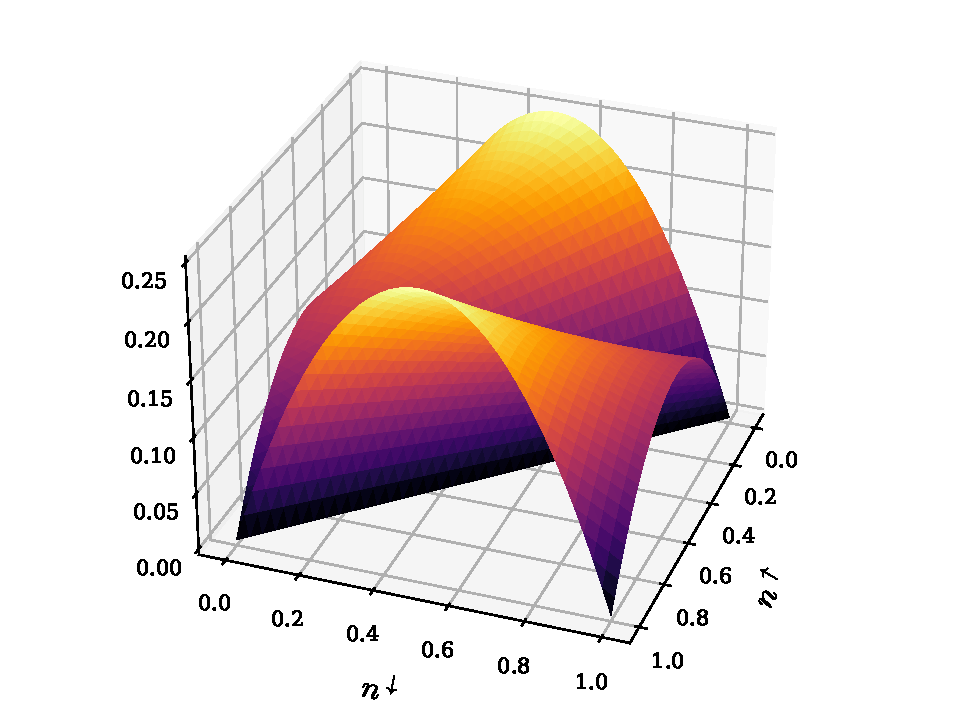
\includegraphics[width=\columnwidth]{figures/novel_u_correction.pdf}
        \end{subfigure}
        \raisebox{2cm}{\huge +}
        \begin{subfigure}[b]{0.4\columnwidth}
            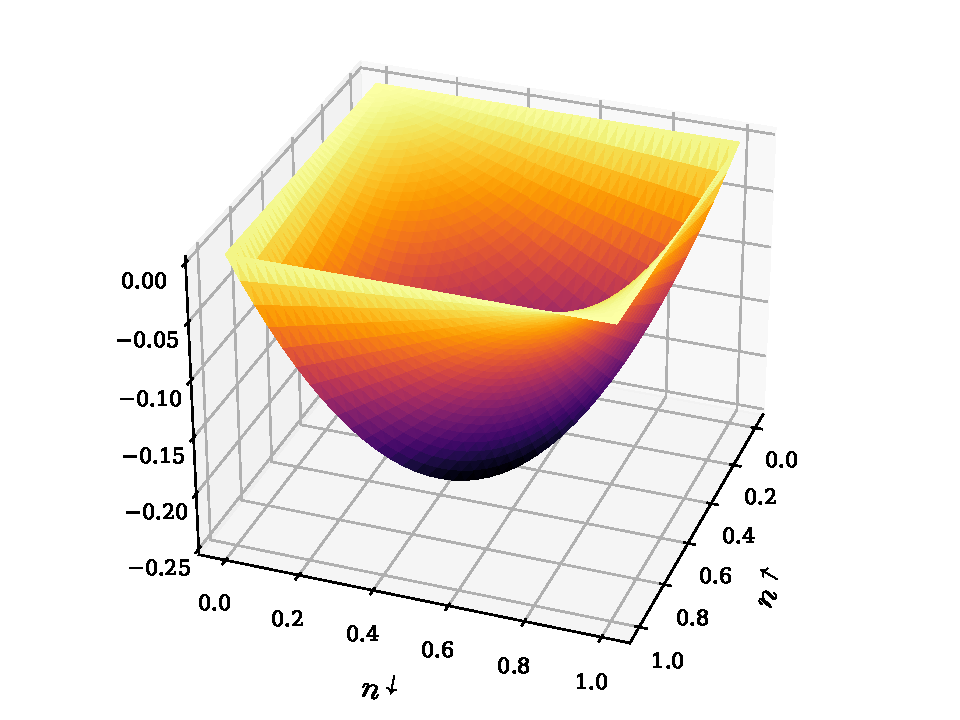
\includegraphics[width=\columnwidth]{figures/novel_k_correction.pdf}
        \end{subfigure}
    \end{figure}

    \footnotesize
    \begin{equation*}
        E_{\mathsf{BLOR}}=\left\{\begin{array}{cc}
            \sum_{\sigma m m^{\prime}} \frac{U^\sigma}{2} n_{m m^\sigma}^\sigma \delta_{m m^{\prime}}-\frac{U^\sigma}{2} n_{m m^{\prime}}^\sigma n_{m^{\prime} m}^\sigma-\frac{U^\sigma+2 J}{2} n_{m m^{\prime}}^\sigma n_{m^{\prime} m}^{\bar{\sigma}},                                                                  & N \leqslant 2 l+1 \\
            \sum_{\sigma m m^{\prime}}\left(U^\sigma+\frac{U^{\bar{\sigma}}}{2}+2 J\right) n_{m m^{\prime}}^\sigma \delta_{m m^{\prime}}-\frac{U^\sigma}{2} n_{m m^{\prime}}^\sigma n_{m^{\prime} m}^\sigma-\frac{U^\sigma+2 J}{2} n_{m m^{\prime}}^\sigma n_{m^{\prime} m}^{\bar{\sigma}}-\frac{U^\sigma+2 J}{2(2 l+1)}, & N>2 l+1
        \end{array}\right.
    \end{equation*}
    % \begin{equation}
    %     v^\sigma(n^\uparrow, n^\downarrow) =
    %     \begin{cases}
    %         {U^\sigma}
    %         \left(\frac{1}{2} - n^\sigma\right)
    %         +
    %         \left(
    %         1 - n^{-\sigma}
    %         \right)
    %         \left(
    %         \frac{U^\uparrow + U^\downarrow}{2}
    %         +K
    %         \right)
    %          & n > 1 \\
    %         U^\sigma
    %         \left(
    %         \frac{1}{2}
    %         -n^{\sigma}
    %         \right)
    %         - n^{-\sigma}
    %         \left(
    %         \frac{U^\uparrow + U^\downarrow}{2}
    %         + K
    %         \right)
    %          & n < 1
    %     \end{cases}
    %     \label{eqn:the_combined_potential}
    % \end{equation}
\end{frame}

\begin{frame}{What's in a name?}
    \begin{center}
        \huge BLOR
    \end{center}
    \begin{center}
        \footnotesize
        \begin{tabularx}{0.7\textwidth}{CCC}
            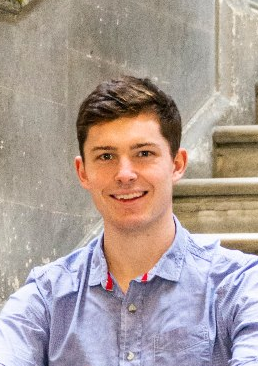
\includegraphics[height = 0.4\paperheight]{photos/andrew_burgess.png} &
            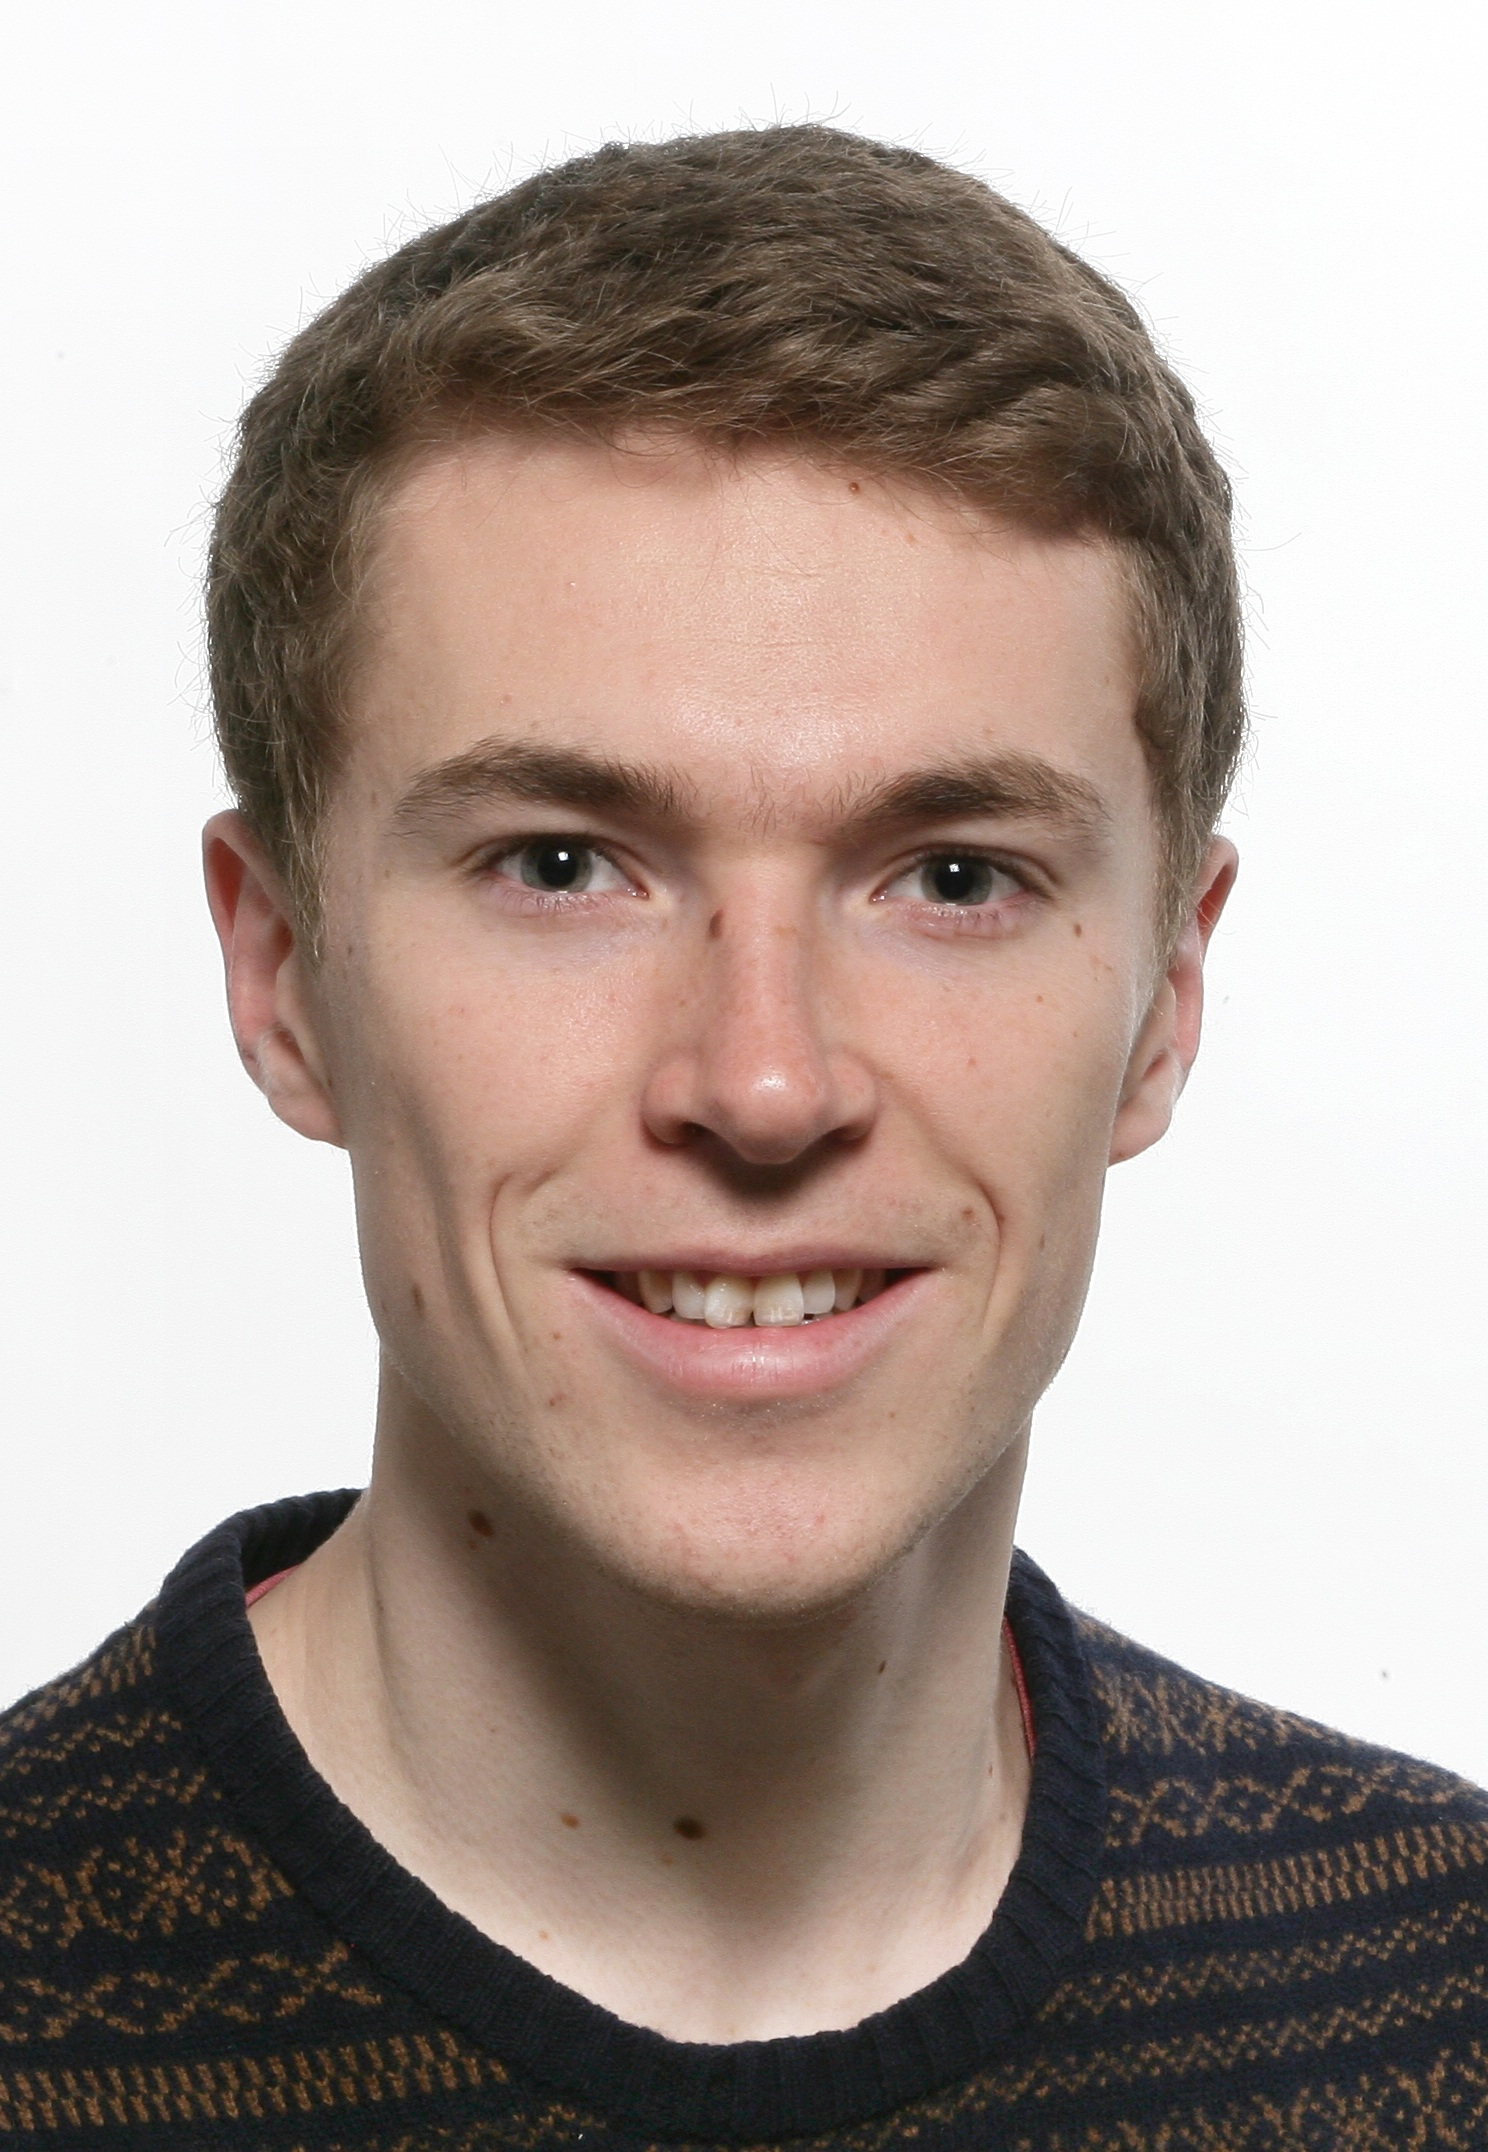
\includegraphics[height = 0.4\paperheight]{photos/linscott.jpg}       &
            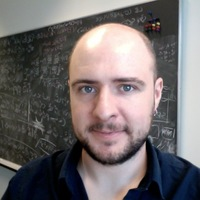
\includegraphics[height = 0.4\paperheight]{figures/david_oregan.jpg}    \\
            % 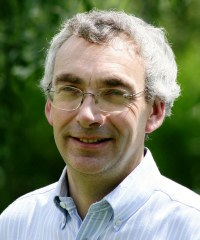
\includegraphics[height = 0.2\paperheight]{figures/mike_payne.jpeg}        &
            % 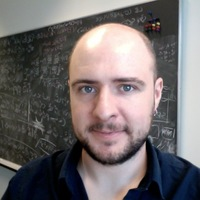
\includegraphics[height = 0.2\paperheight]{figures/david_oregan.jpg}         \\
            Andrew \only<2->{\textbf}{B}urgess                                    &
            Edward \only<2->{\textbf}{L}inscott                                   &
            David \only<2->{\textbf}{O}'\only<2->{\textbf}{R}egan                   \\
        \end{tabularx}
    \end{center}

    \onslide<3->{Initially was going to be ``BLR22'' but...}
\end{frame}

\begin{frame}{What's in a name?}
    \centering
    \only<1-2>{
        \begin{tikzpicture}
            \only<1>{\node[anchor=center] at (0,0) {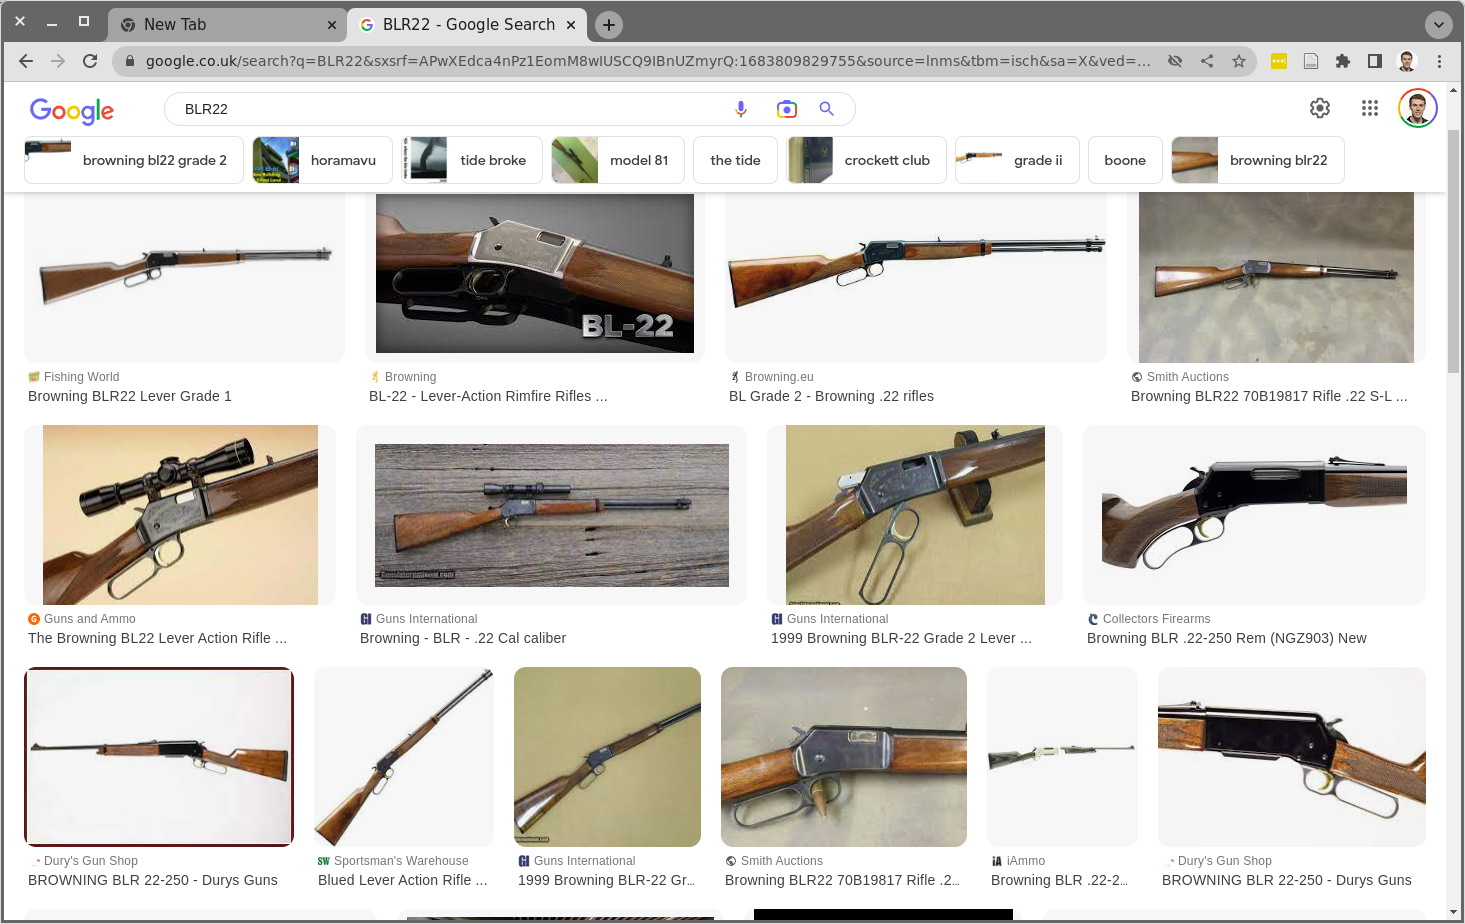
\includegraphics[width=0.9\textwidth]{figures/blr22.png}}};
            \only<2>{\node[opacity=0.3, anchor=center] at (0,0) {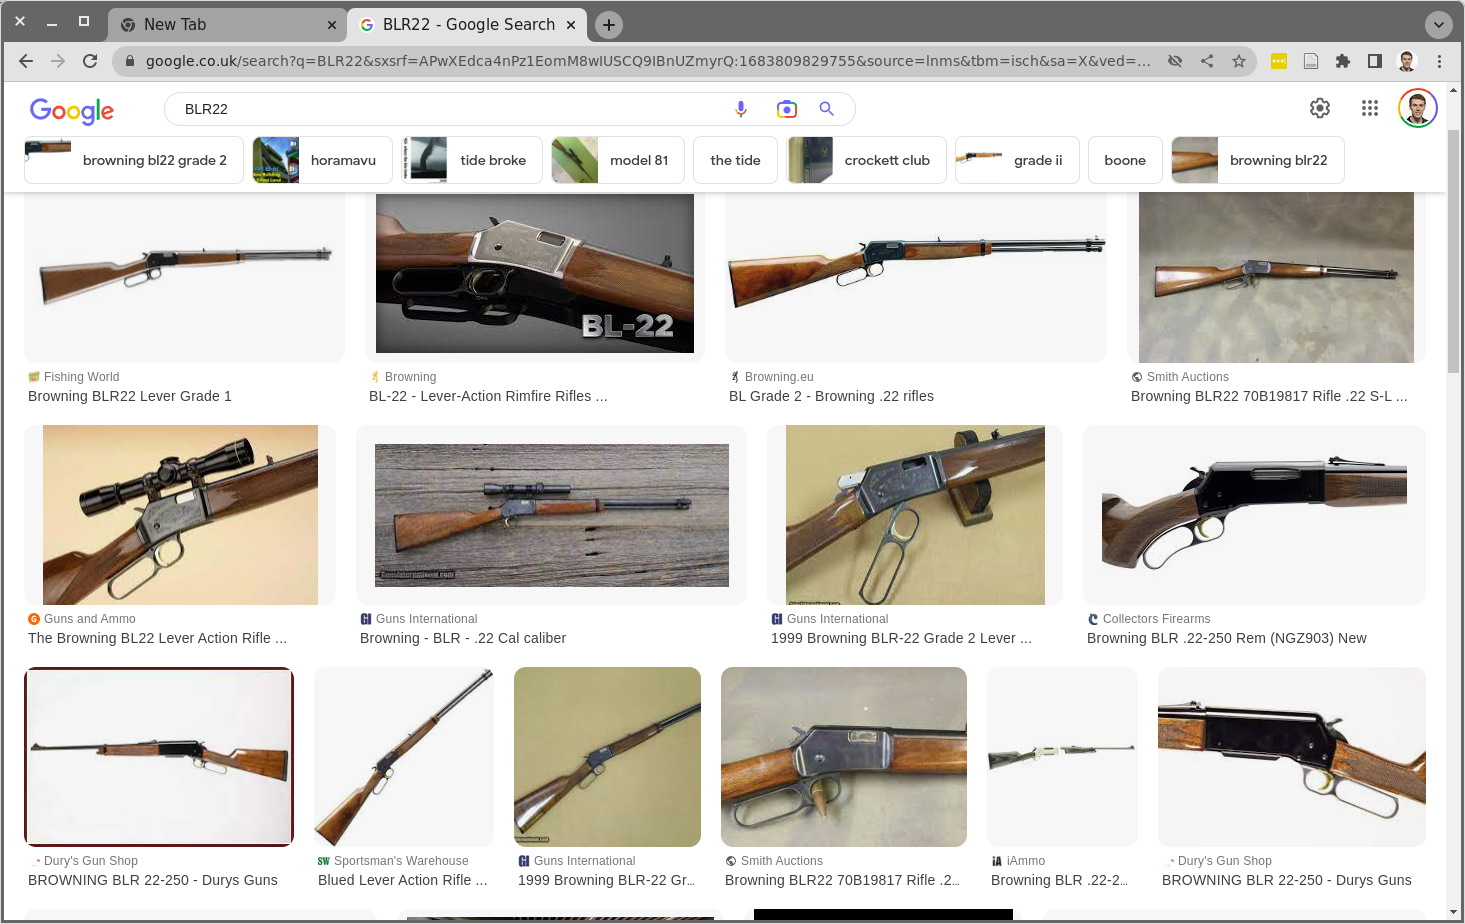
\includegraphics[width=0.9\textwidth]{figures/blr22.png}}};
            \only<2->{\node[anchor=center] at (0,0) {\Large when naming something, ALWAYS Google it first!}};
        \end{tikzpicture}
    }

\end{frame}
% %
% \Cref{eqn:the_combined_potential} is one of the main results of this work. The first term is the familiar conventional +\emph{U} potential with a spin-dependent $U$. The second term is less familiar. It introduces a $n^{-\sigma}$-dependent shift with a discontinuity across $n = 1$ of magnitude
% %
% \begin{equation}
% \lim_{n\rightarrow 1^+} v^\sigma
% - \lim_{n\rightarrow 1^-} v^\sigma
% = 
%     \frac{U^\uparrow + U^\downarrow}{2}
%     + K
% \end{equation}
% %
% I need to think more to understand this discontinuity and its origins. Additionally, the particular combination of the parameters $\frac{U^\uparrow + U^\downarrow}{2} + K$ is important. Note that if we set $K = -\frac{U^\uparrow + U^\downarrow}{2}$ we return to conventional DFT\,+\,\emph{U}. (This corresponds to deploying the $K$-correction to add back in the curvature with respect to $\mu$ that the conventional $+U$ correction erroneously includes but my $+U$ correction correctly does not possess.)
% 
% I worry that this discontinuity will lead to strange behaviour and thereby render my correction unusable. 
% 
% \section{Determining $U^\sigma$ and $K$ via linear response}
\begin{frame}{Determining $U^\sigma$ and $J$ via spin-resolved LR}

    Scalar (conventional) approach:
    \begin{align*}
        \chi_{IJ} = & \frac{d n^I}{d v^J_\mathsf{ext}}\qquad \hat v^J_\mathsf{ext} = v_\mathsf{ext} \hat P^J
    \end{align*}
    %

    Spin-resolved approach\footcite{Linscott2018}:
    \begin{align*}
        \chi_{IJ\sigma\sigma'} = & \frac{d n^{I\sigma}}{d v^{J\sigma'}_\mathsf{ext}}\qquad \hat v^{J\sigma}_\mathsf{ext} = \delta_{\sigma \sigma'} v^{\sigma'}_\mathsf{ext} \hat P^J
    \end{align*}

    Allows us to construct perturbations while holding variables constant without a headache e.g. $\left.\frac{d}{dn^\uparrow}\right|_{n^\downarrow}$

\end{frame}

\begin{frame}{Does BLOR work? Stretched H\textsuperscript{5+}}
    \begin{center}
        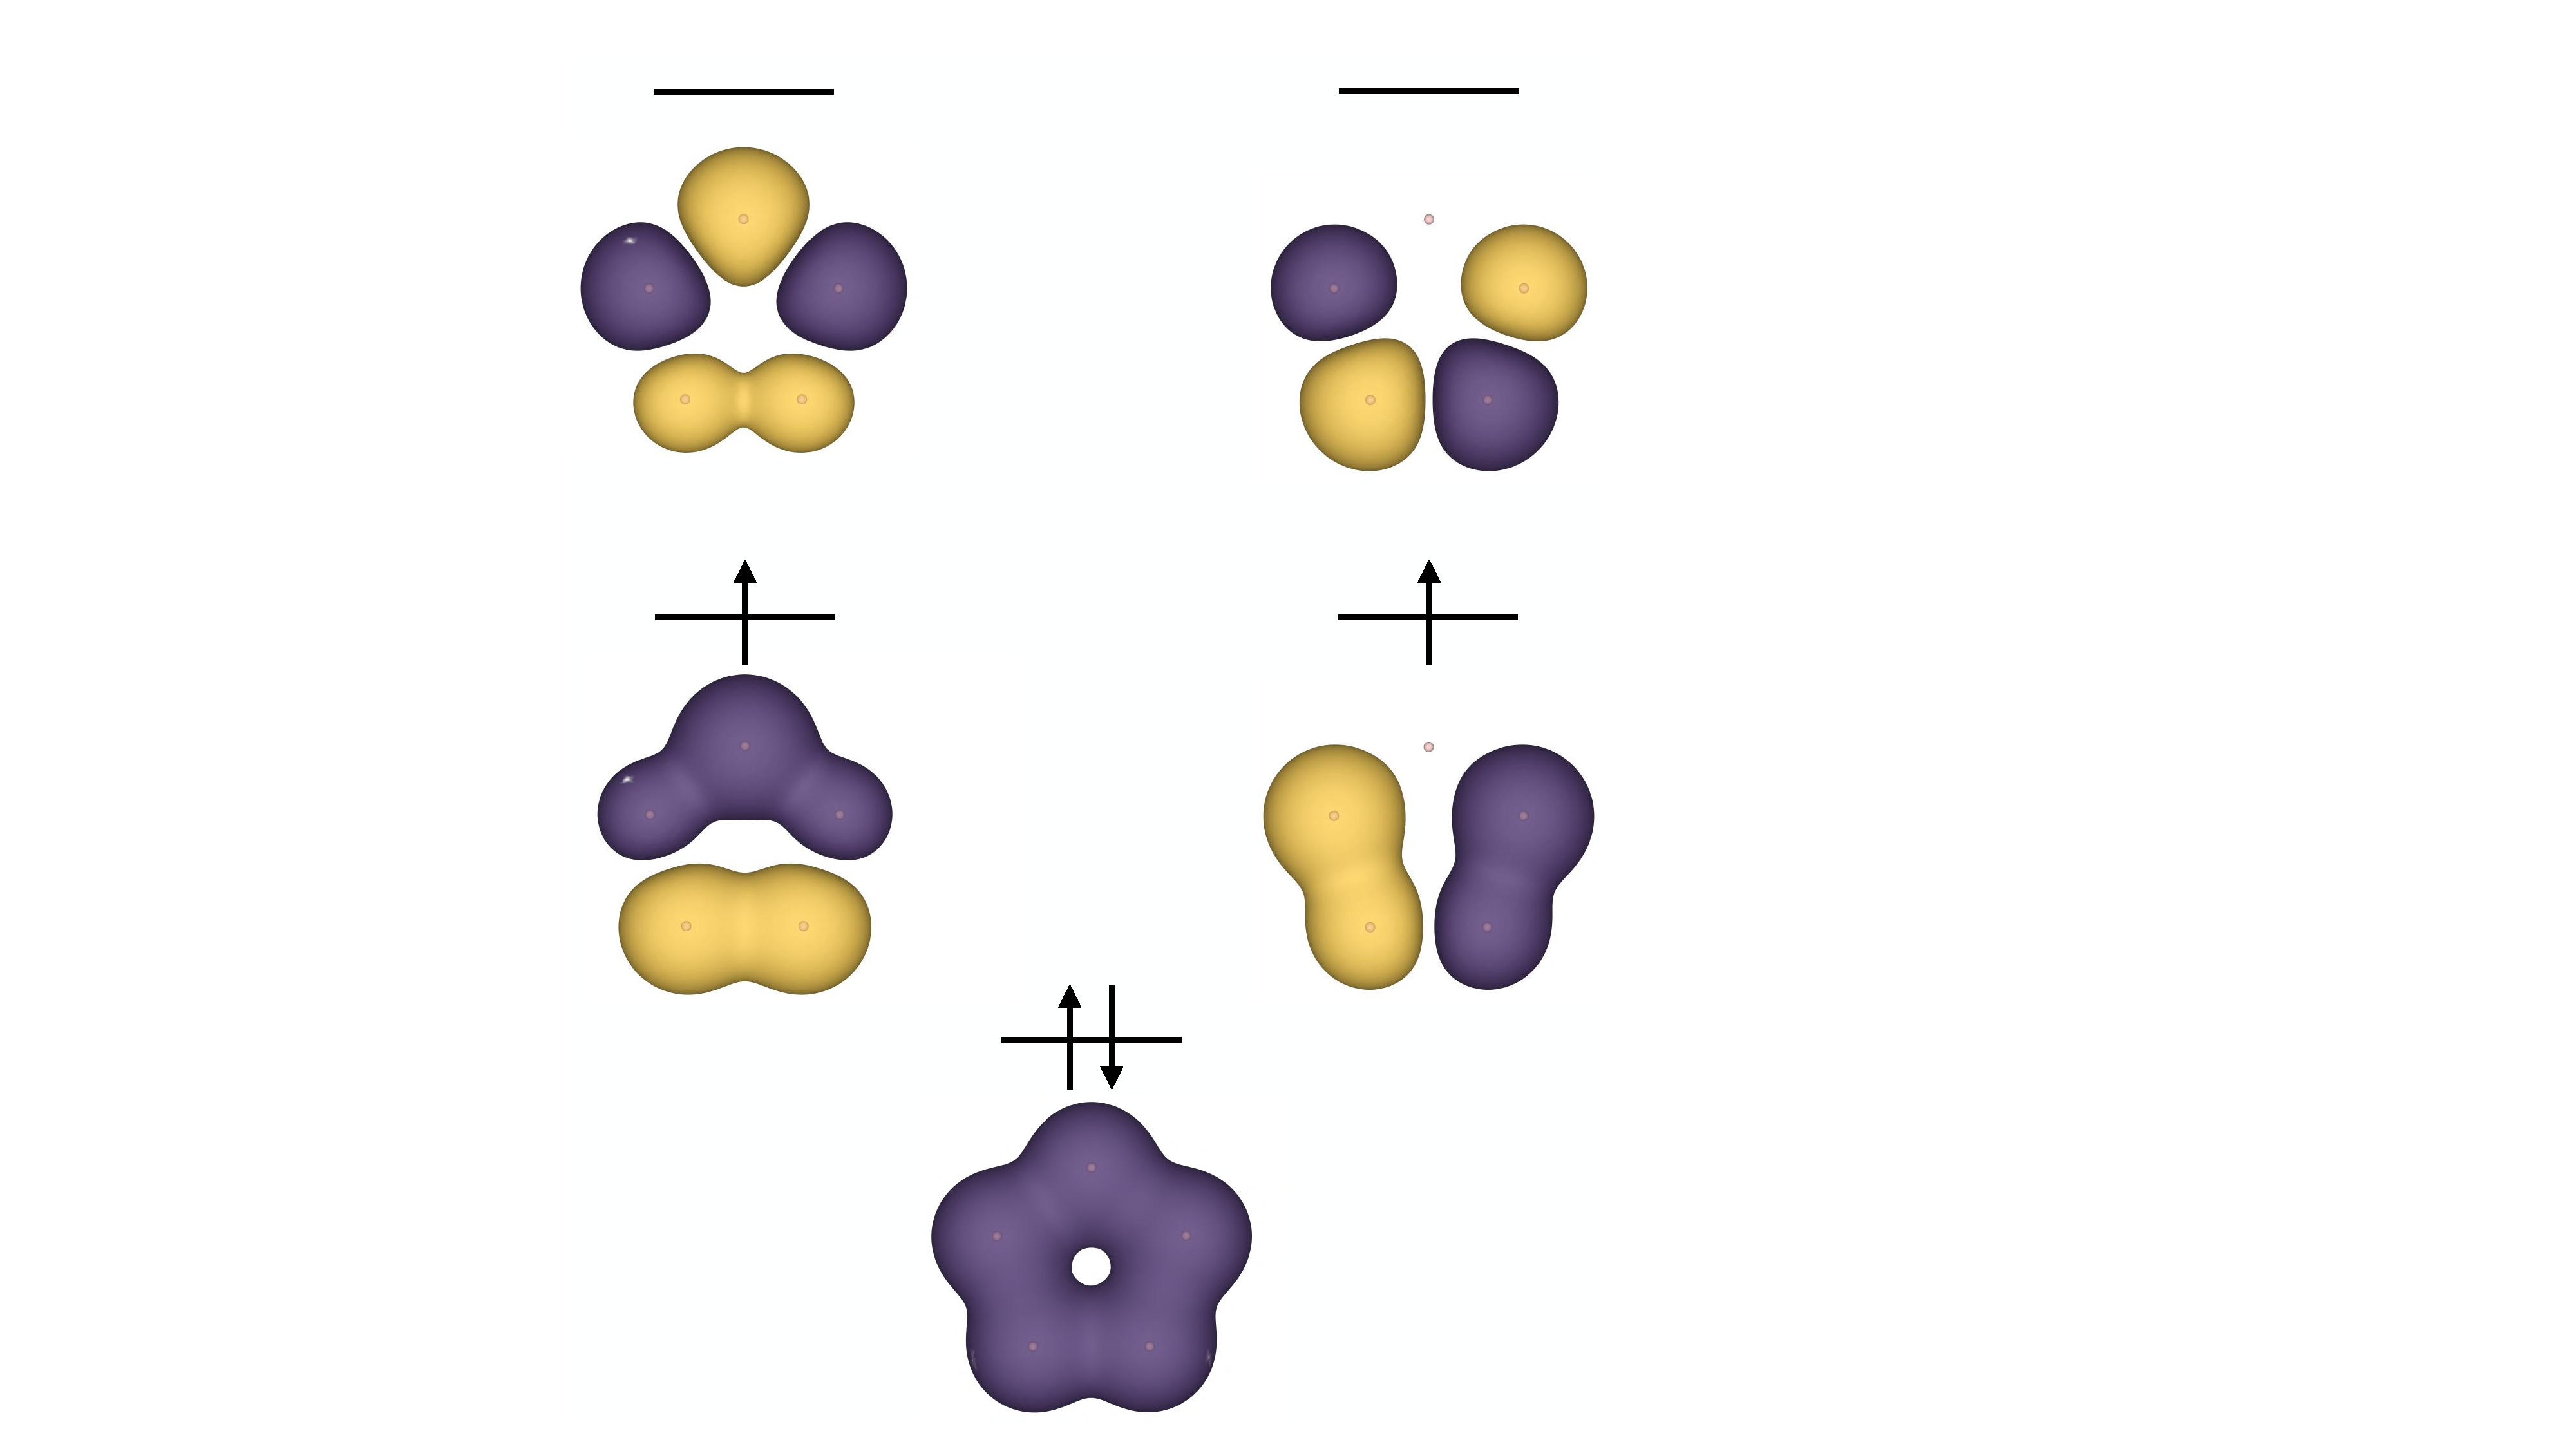
\includegraphics[height=0.8\textheight]{figures/burgess/mo3.pdf}
        \hspace{0.05\textwidth}
        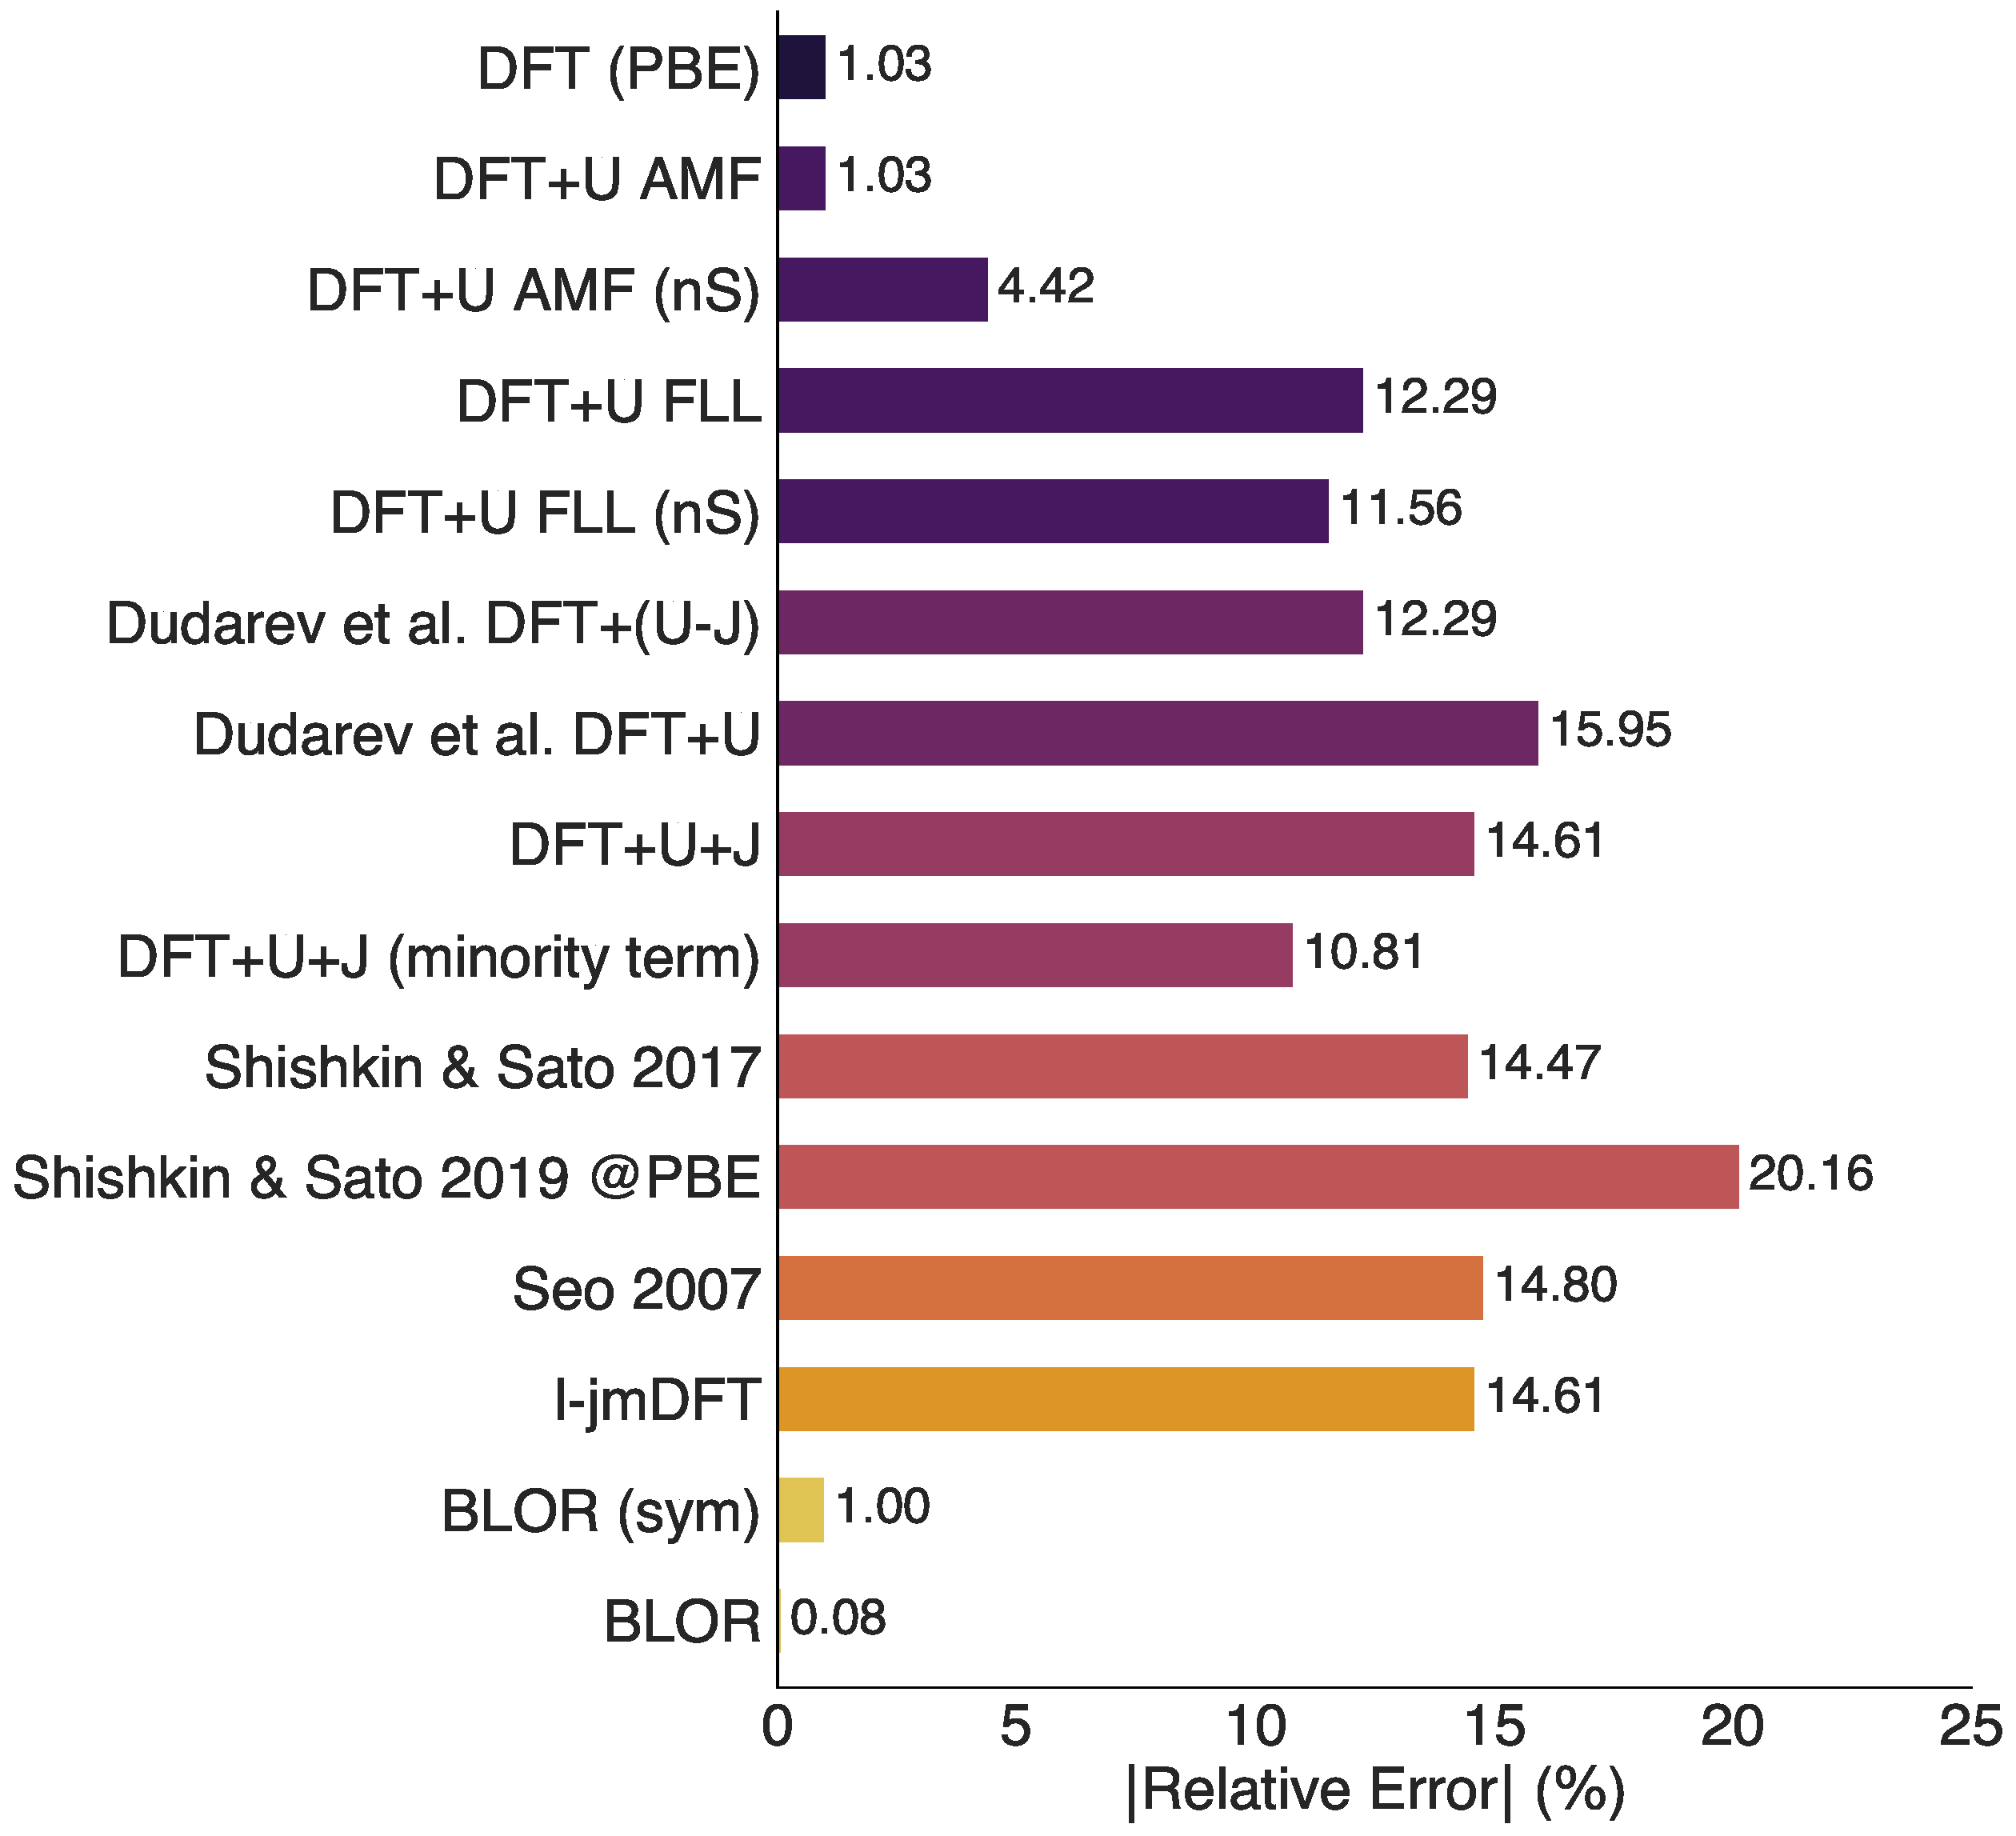
\includegraphics[height=0.8\textheight]{figures/burgess/h5+_extended.pdf}
    \end{center}
\end{frame}

\begin{frame}{Does BLOR work?}
    \begin{tabularx}{0.9\textwidth}{CC}
        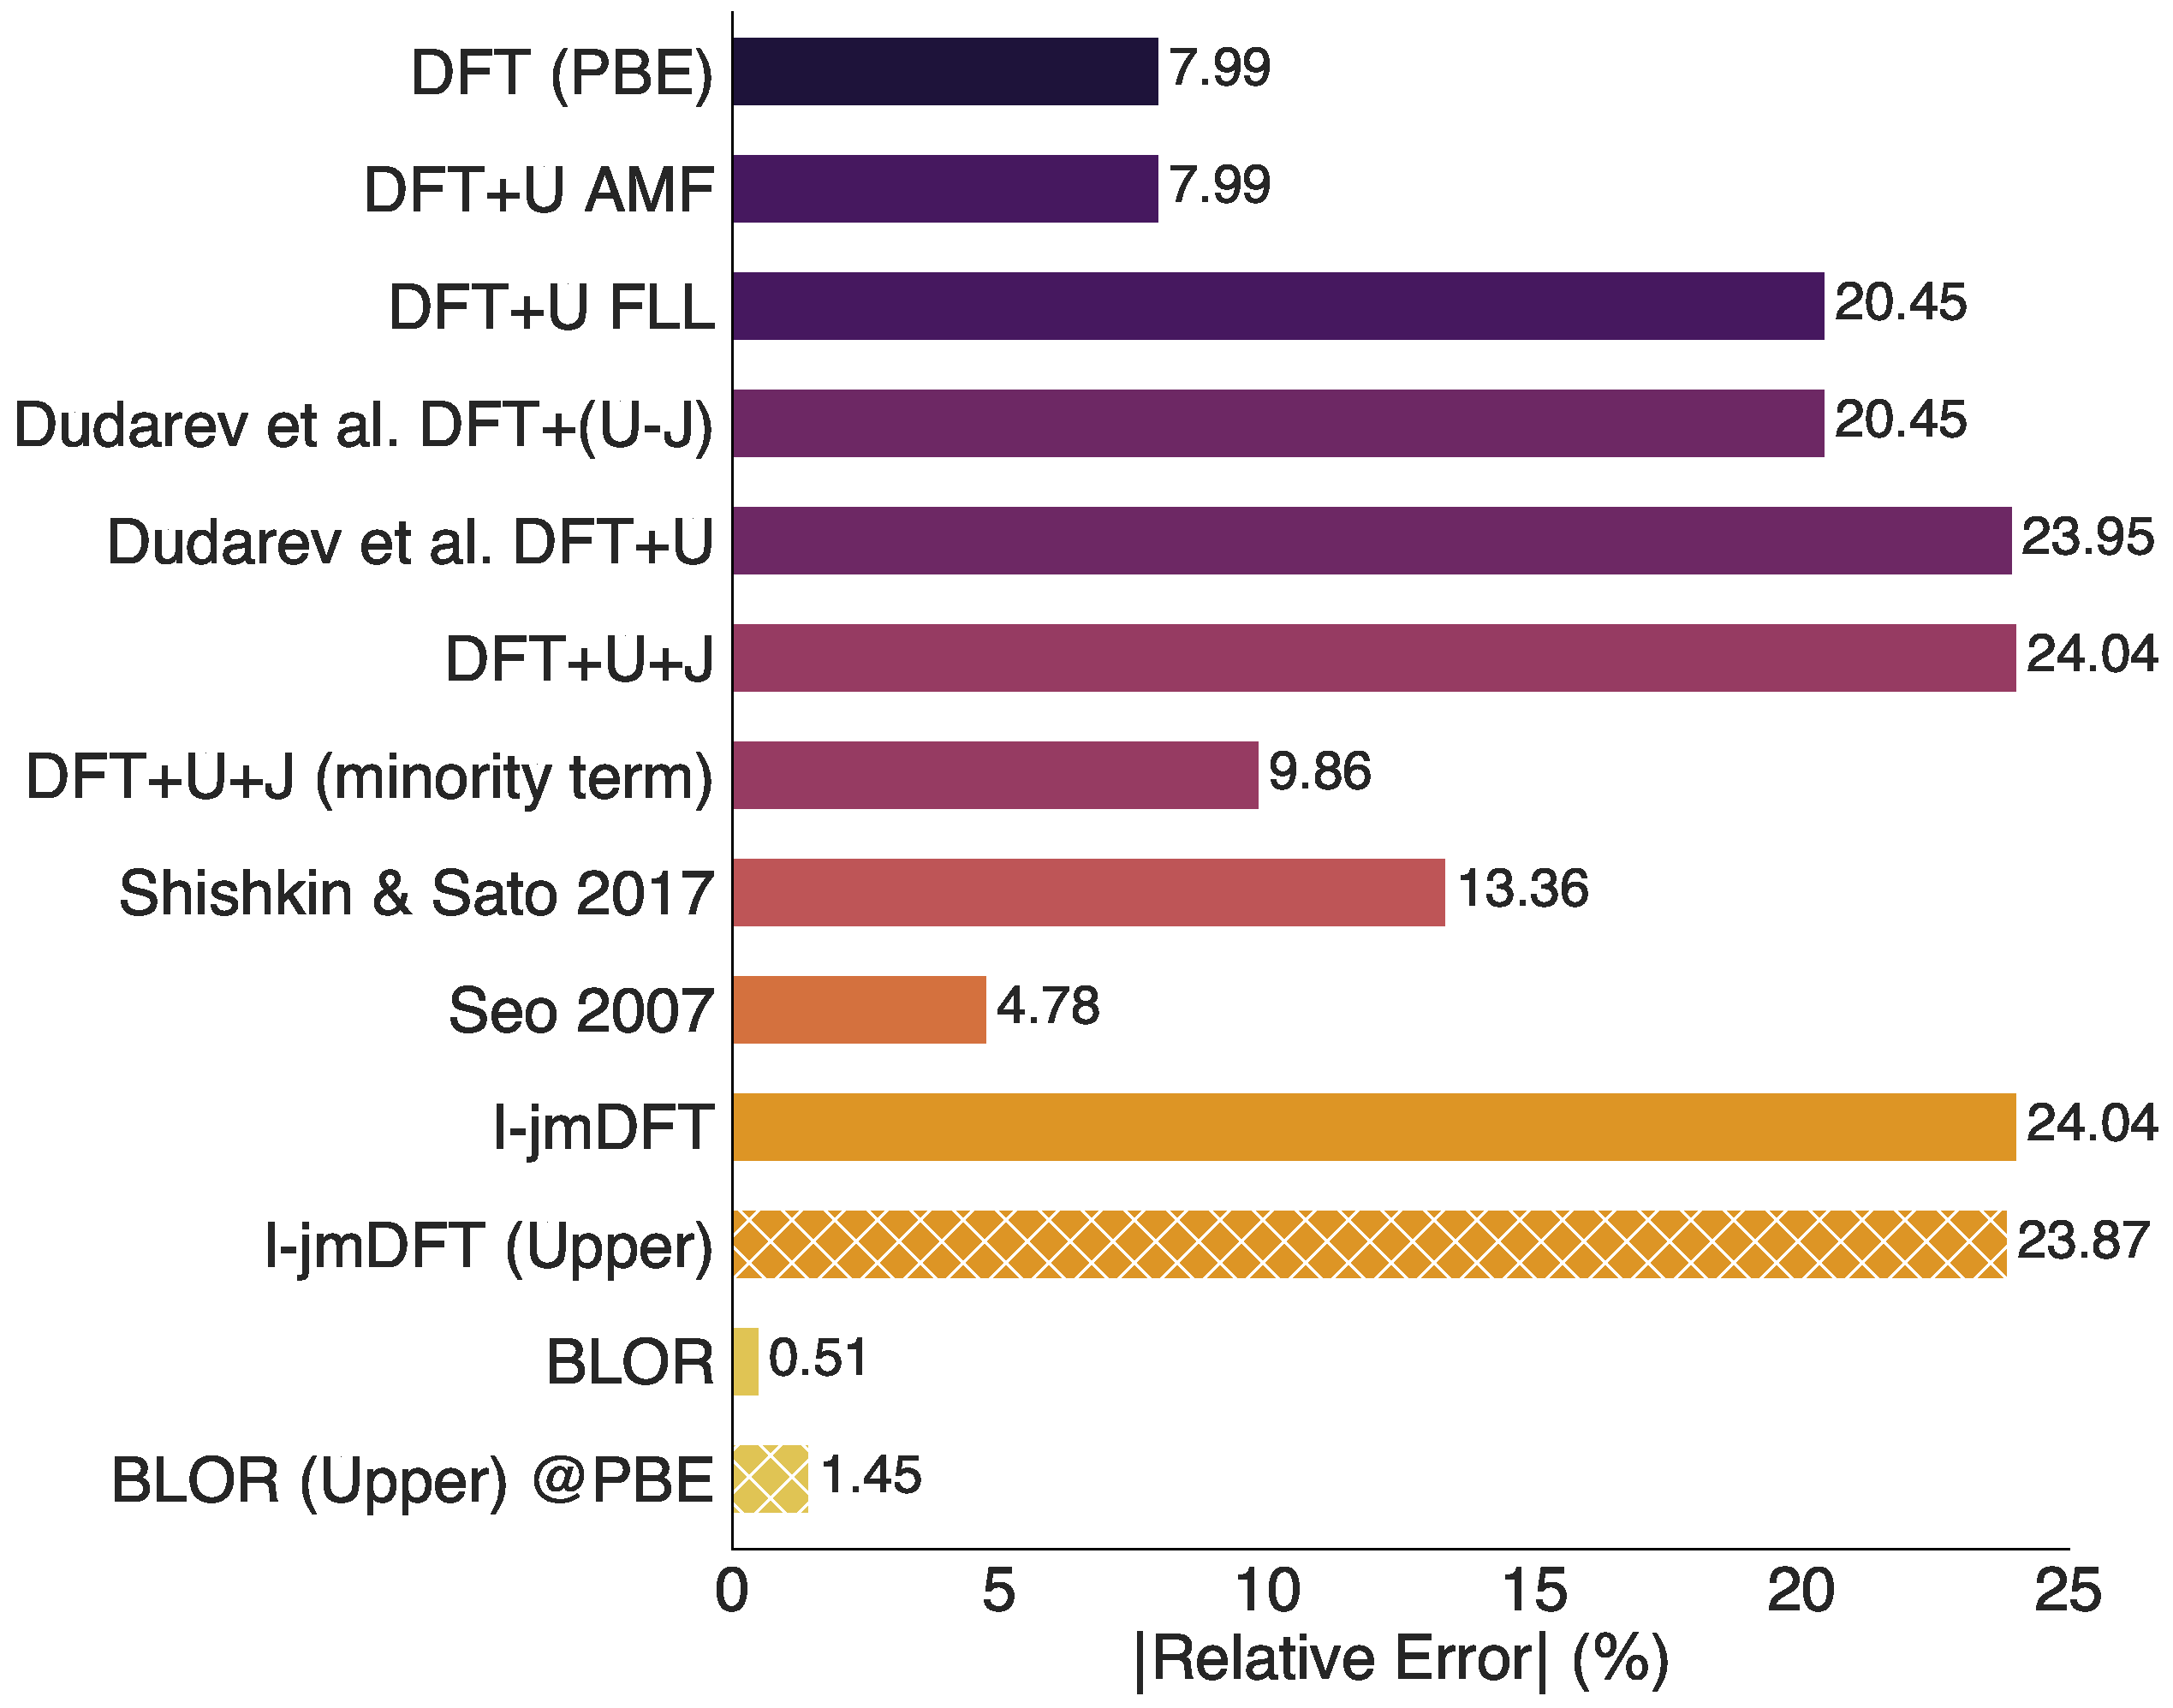
\includegraphics[height=0.6\textheight]{figures/burgess/h2_extended.pdf} &
        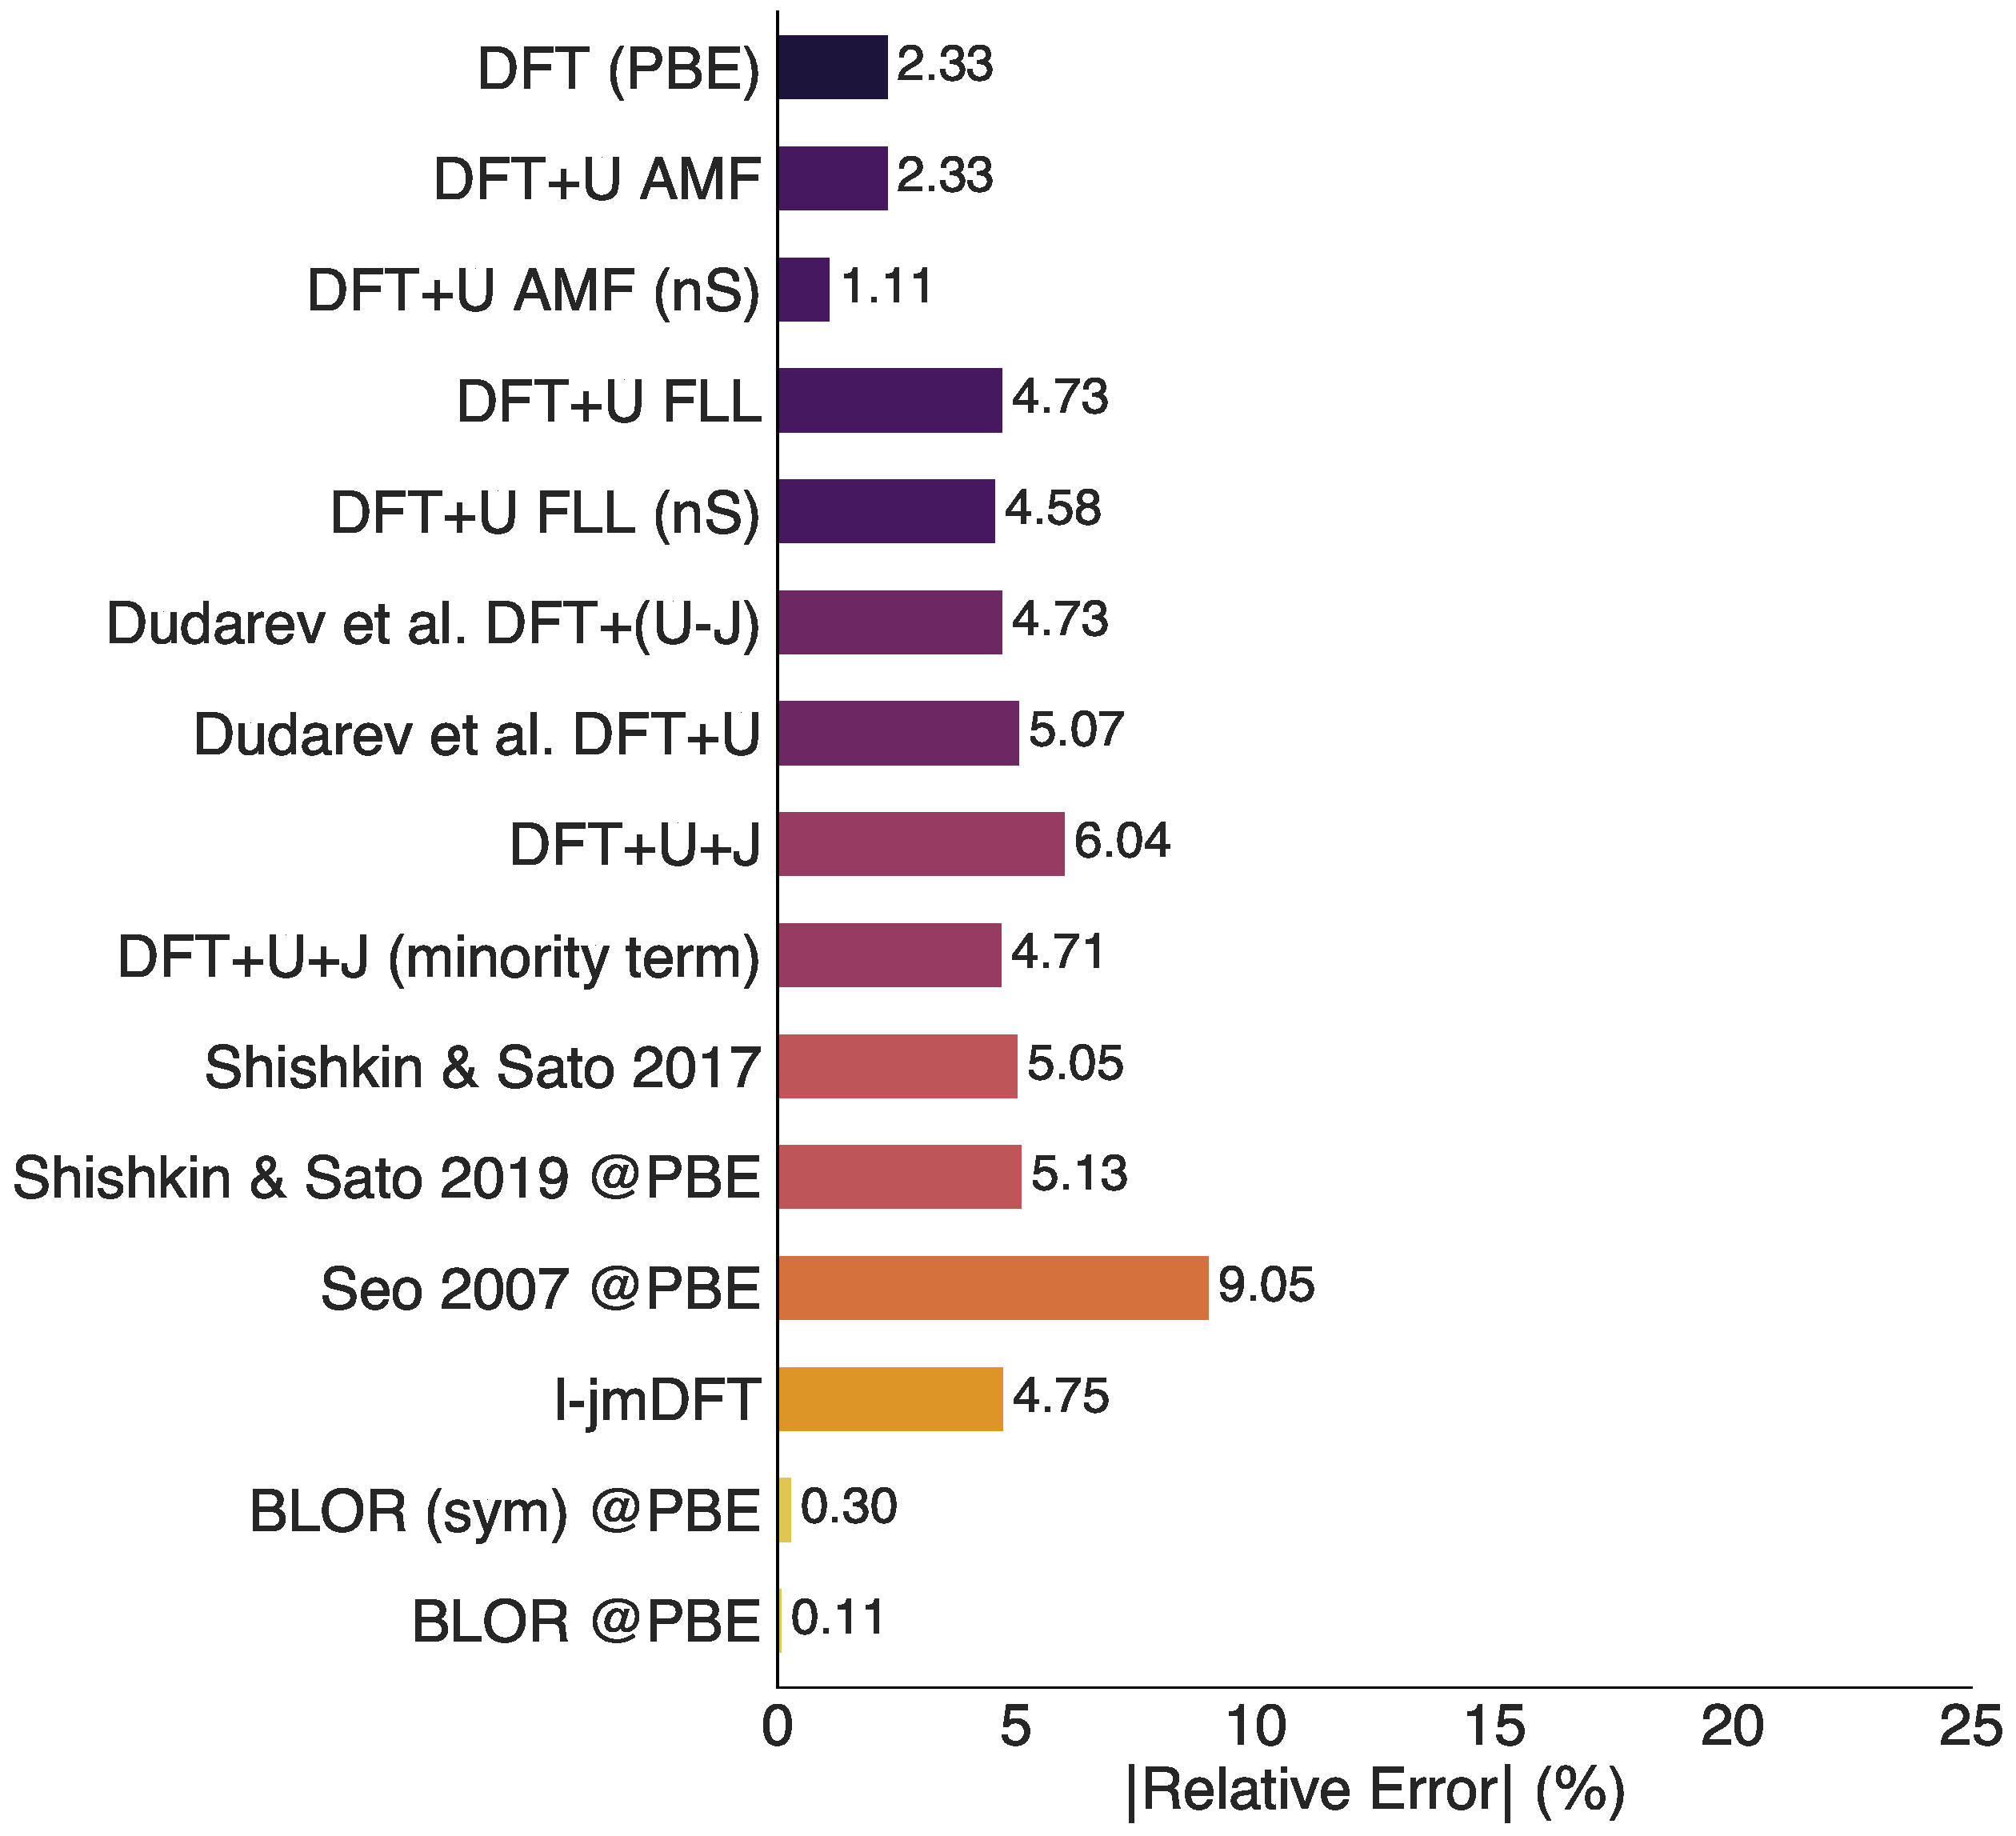
\includegraphics[height=0.6\textheight]{figures/burgess/He2+.pdf}          \\
        stretched H\textsubscript{2}                                             &
        stretched He$_2^+$                                                         \\
    \end{tabularx}
\end{frame}

\begin{frame}{Does BLOR work?}
    \begin{tabularx}{0.9\textwidth}{CC}
        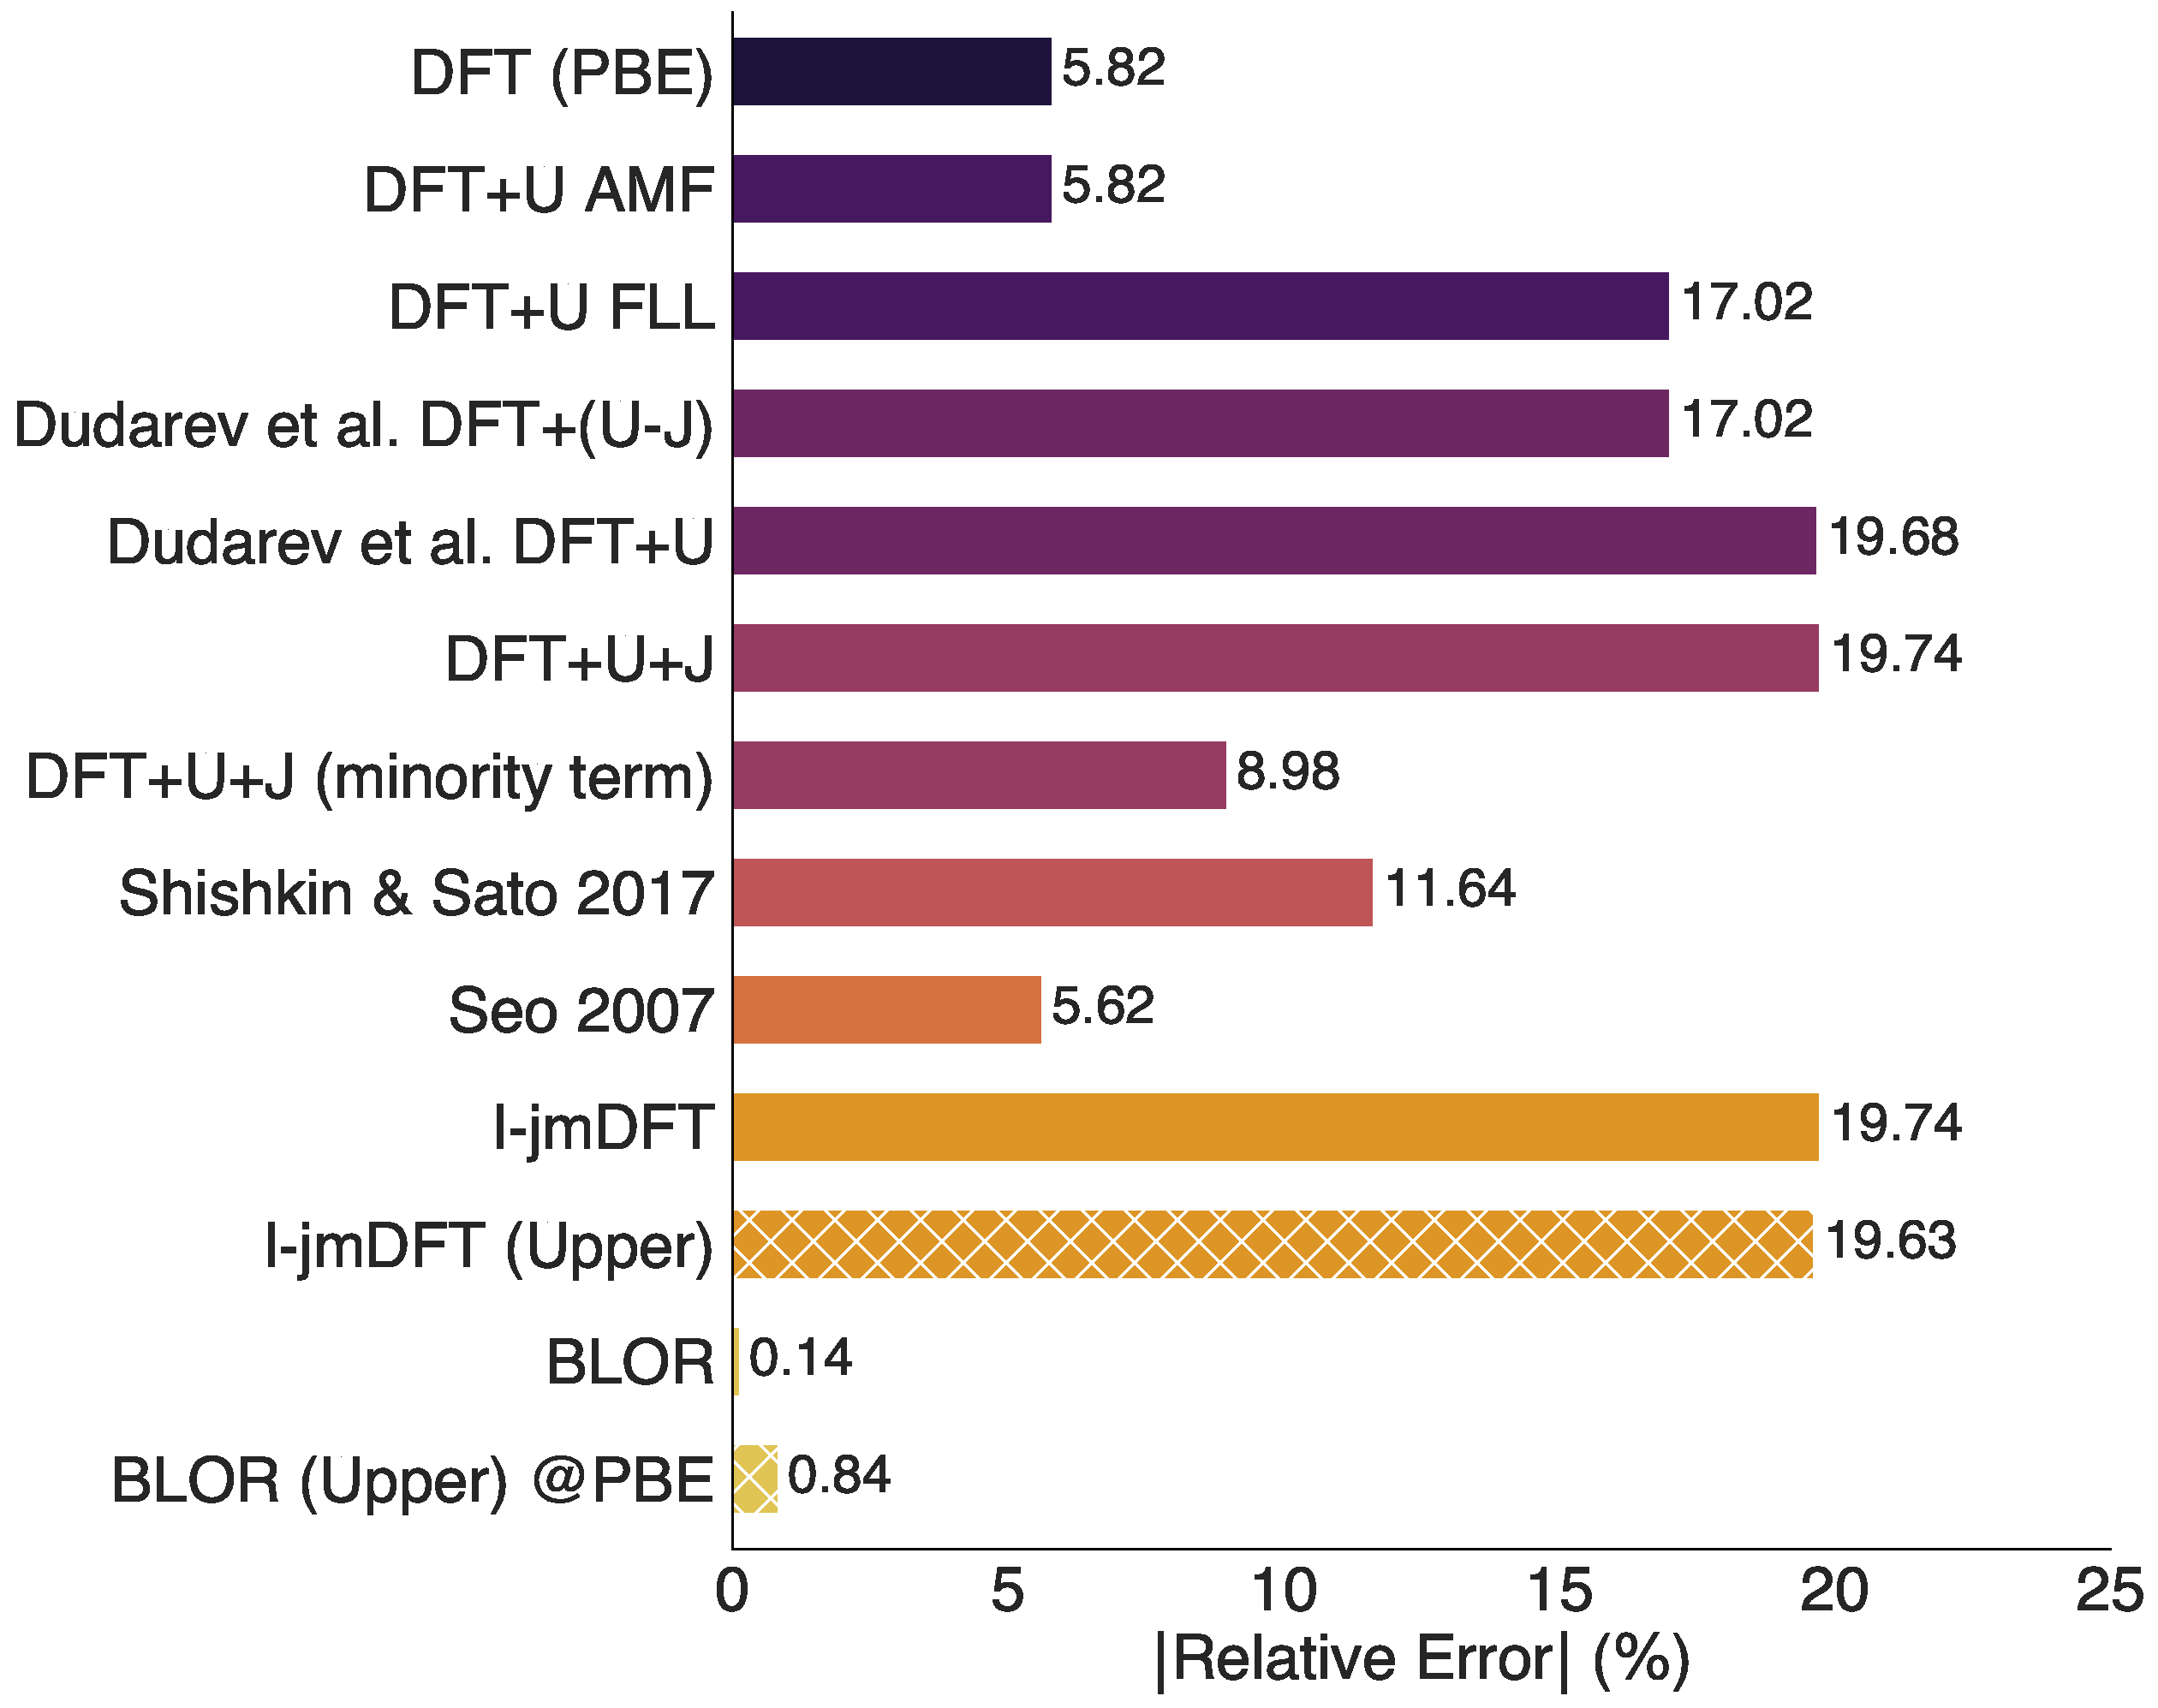
\includegraphics[height=0.6\textheight]{figures/burgess/Li2.pdf} &
        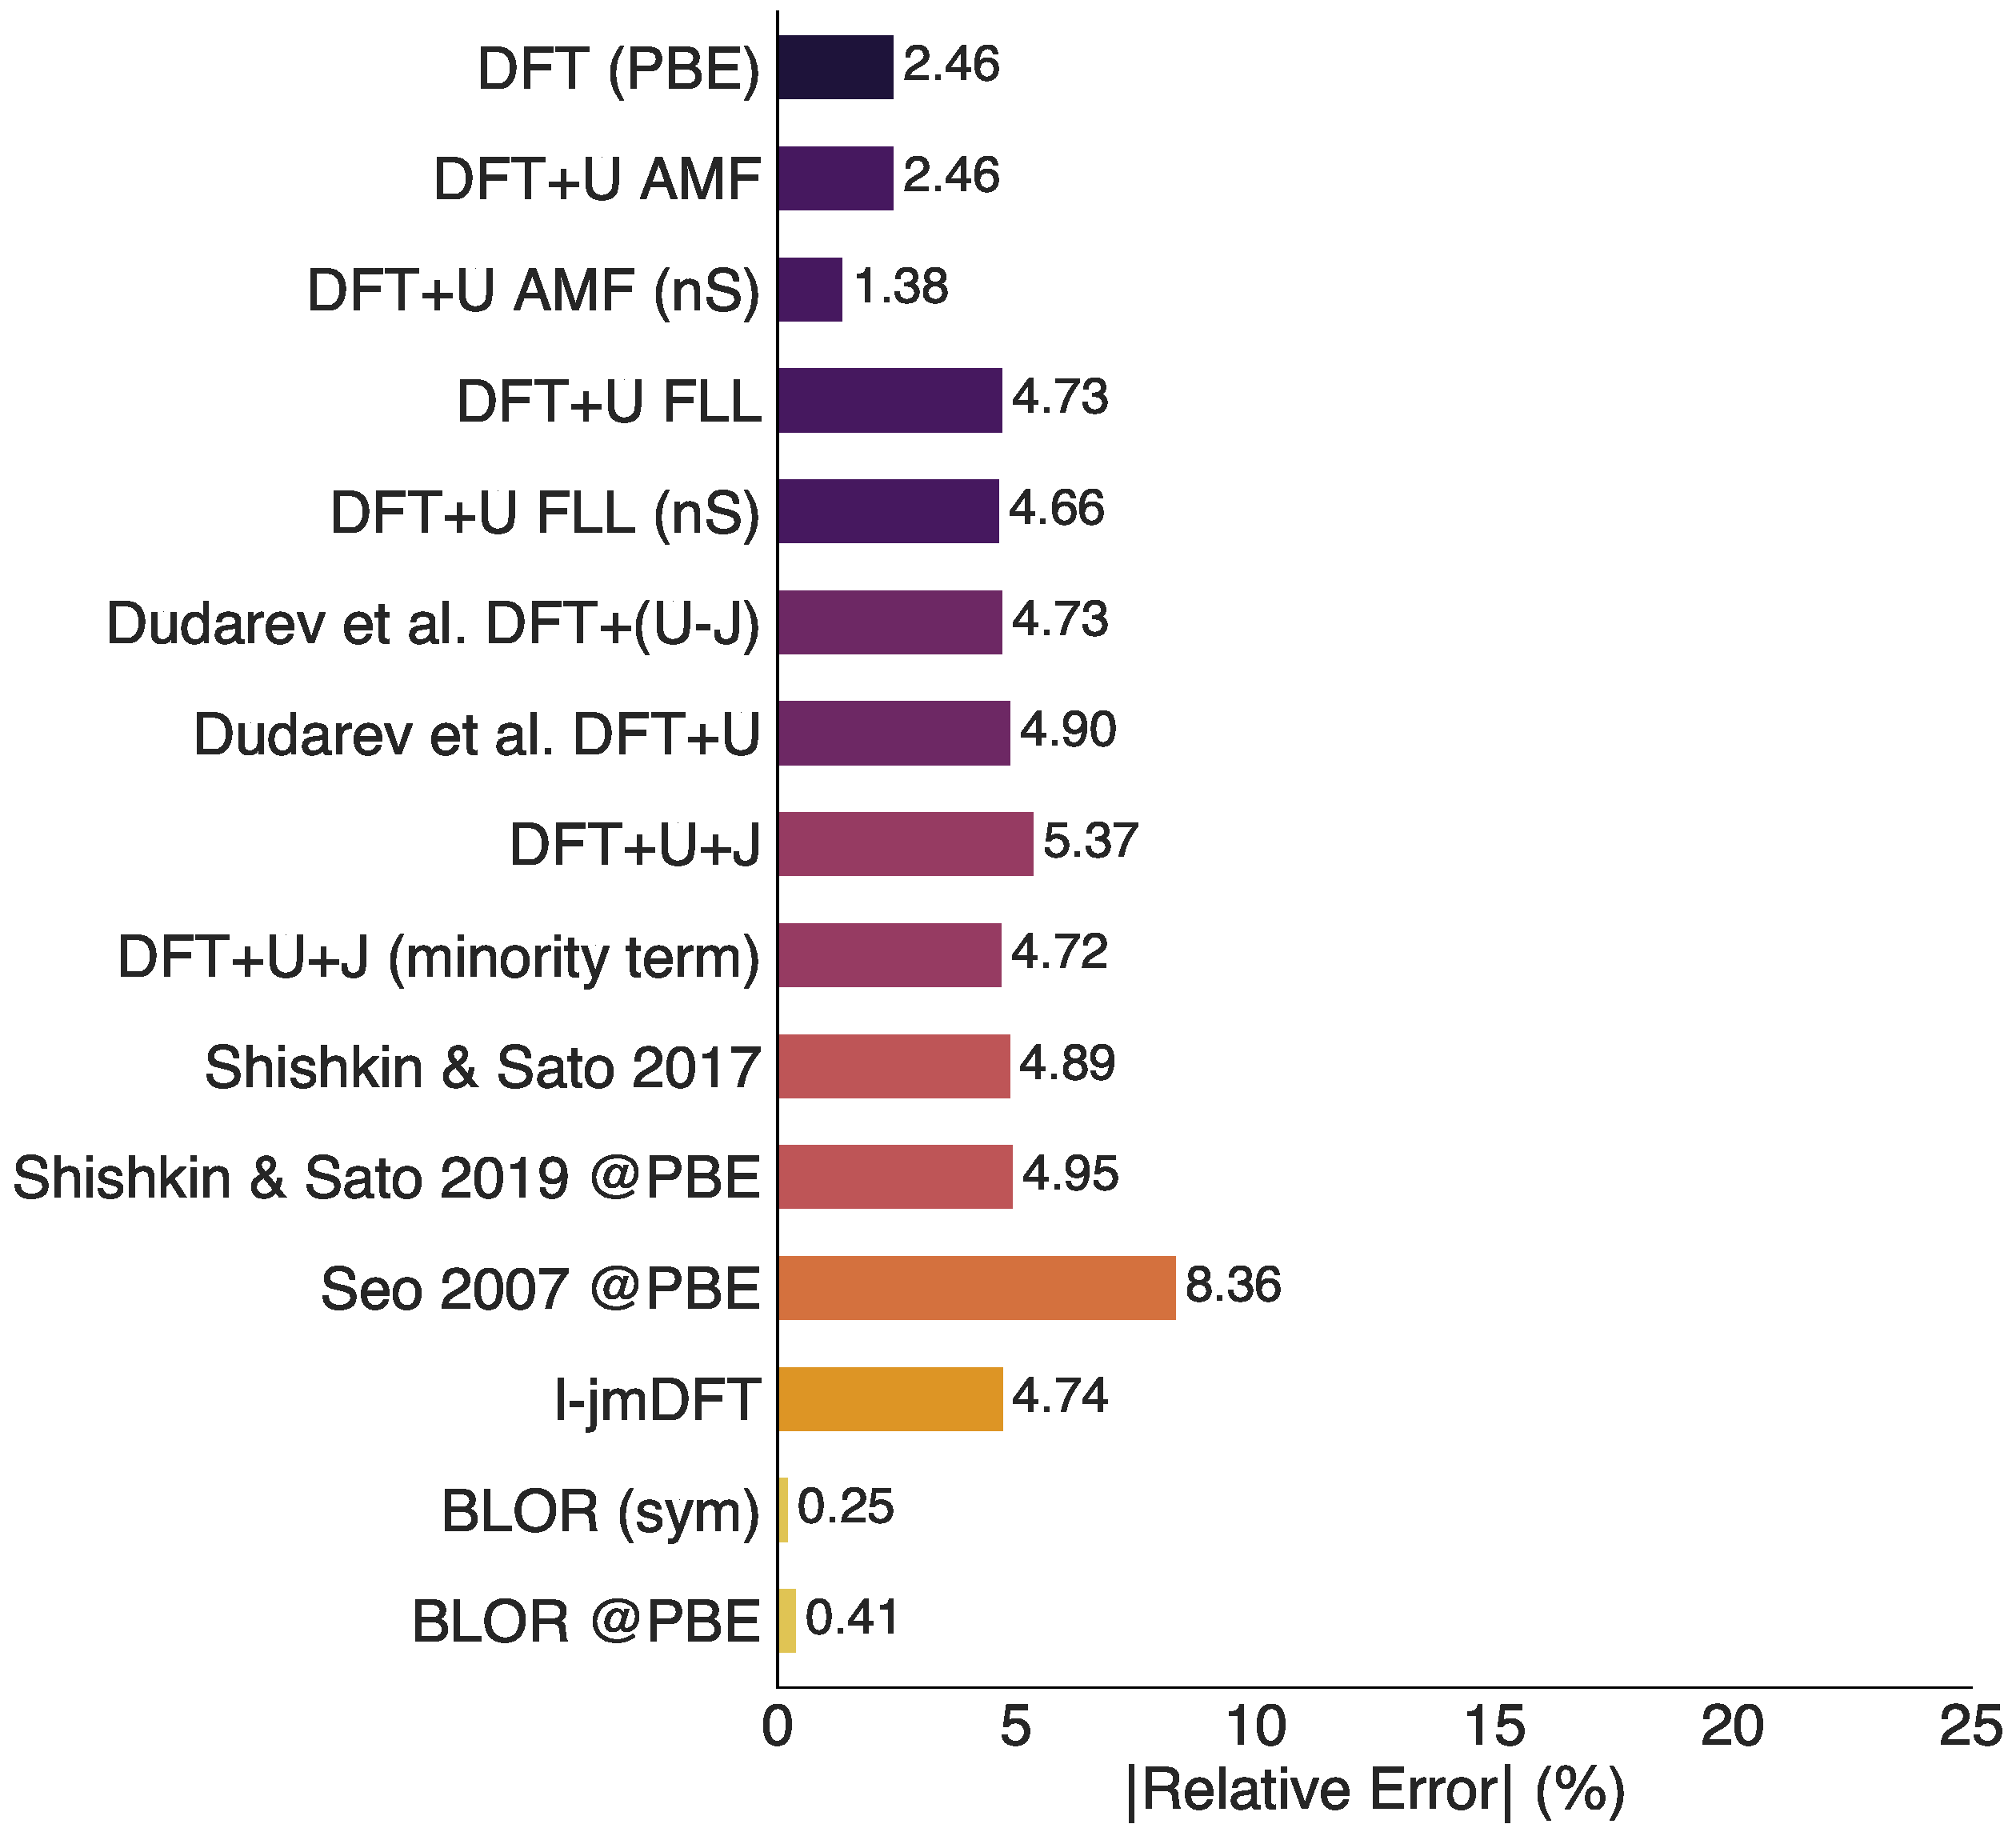
\includegraphics[height=0.6\textheight]{figures/burgess/Be2+.pdf}  \\
        stretched Li\textsubscript{2}                                    &
        stretched Be$_2^+$                                                 \\
    \end{tabularx}
\end{frame}

\begin{frame}{Conclusions}
    \begin{itemize}
        \item we can get excellent total energies when we take the mandate of the flat plane seriously
        \item BUT still many important details to be worked out...
    \end{itemize}

\end{frame}

\begin{frame}{``Potential'' issues...}
    The resulting potential from the SIE energy correction is given by $\hat v^\sigma_1 = v^\sigma_1(n^\uparrow_i, n^\downarrow_i) \ket{i}\bra{i}$ where
    %
    \begin{columns}
        \column{0.5\textwidth}
        \small
        \begin{align*}
            v^\sigma_1(n^\uparrow, n^\downarrow)
            % = -\frac{\tilde n U^\sigma}{2} + \sum_{\sigma'} \frac{U^{\sigma'}}{4} \left[\frac{|\tilde n|}{\tilde n} + 1 - 2n^{\sigma'}\right]
            = &
            \begin{cases}
                U^\sigma\left(\frac{1}{2} - n^\sigma\right)
                + \left(1 - n^{-\sigma}\right)
                \frac{U^\uparrow + U^\downarrow}{2}
                 & n > 1
                \\
                U^\sigma\left(\frac{1}{2} - n^\sigma\right)
                - n^{-\sigma}
                \frac{U^\uparrow + U^\downarrow}{2}
                 & n < 1
            \end{cases}
            \label{eqn:novel_u_potential}
        \end{align*}

        \vspace{6pt}
        $\rightarrow$ issues for single-particle energies?

        \vspace{6pt}
        Numerically, can either adopt some smoothing OR Hund's rule comes to the rescue

        \vspace{6pt}
        Other issues include local vs global curvature

        \column{0.4\textwidth}
        \begin{figure}[t!]
            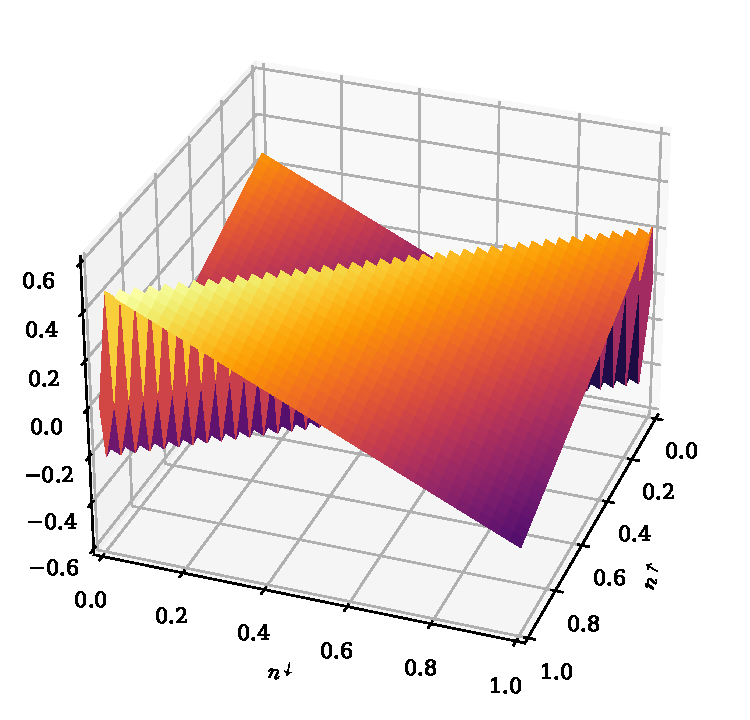
\includegraphics[width=\columnwidth]{figures/novel_u_potential.pdf}
            \label{fig:novel_u_potential}
        \end{figure}
    \end{columns}

\end{frame}

\begin{frame}{Acknowledgements}

    \begin{center}
        \footnotesize
        \begin{tabularx}{0.5\textwidth}{CC}
            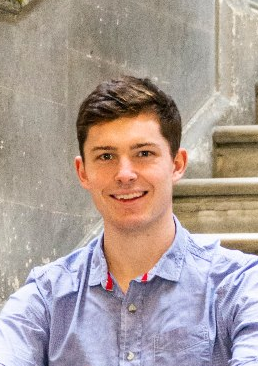
\includegraphics[height = 0.4\paperheight]{photos/andrew_burgess.png} &
            \includegraphics[height = 0.4\paperheight]{figures/david_oregan.jpg}    \\
            % \includegraphics[height = 0.2\paperheight]{figures/daniel_cole.jpeg}       &
            % \includegraphics[height = 0.2\paperheight]{figures/mike_payne.jpeg}        &
            % \includegraphics[height = 0.2\paperheight]{figures/david_oregan.jpg}         \\
            Andrew Burgess                                                        &
            David O'Regan                                                           \\
        \end{tabularx}
    \end{center}

    \vspace{1ex}
    \begin{center}
        paper available at PRB 107, L121115 (2023) | slides available at \includegraphics[height=\fontcharht\font`\B]{logos/github-favicon.png} elinscott (and the wiki!)
    \end{center}


    % \begin{multicols}{2}
    %    \tiny
    %    \printbibliography
    %    \normalsize
    % \end{multicols}
    \vspace{2ex}
    \scriptsize

    \setbeamercolor*{bibliography entry title}{fg=black}
    \setbeamercolor*{bibliography entry author}{fg=black}
    \setbeamercolor*{bibliography entry location}{fg=black}
    \setbeamercolor*{bibliography entry note}{fg=black}

    \vspace{2ex}
    \scriptsize
\end{frame}

% \backupbegin
% \begin{frame}{}
% 
%     \begin{center}
%         \huge SPARE SLIDES
%     \end{center}
% 
% \end{frame}
% 
% \begin{frame}{Spare slide}
% \end{frame}
% 
% 
% \backupend
\end{document}